\documentclass[a4paper, 12pt]{article}

% packages
\usepackage{amssymb}
\usepackage[fleqn]{mathtools}
\usepackage{tikz}
\usepackage{enumerate}
\usepackage{bussproofs}
\usepackage{xcolor}
\usepackage[margin=1.3cm]{geometry}
\usepackage{logicproof}
\usepackage{diagbox}
\usepackage{listings}
\usepackage{graphicx}
\usepackage{lstautogobble}
\usepackage{hyperref}
\usepackage{multirow}
\usepackage{tipa}
\usepackage{pgfplots}
\usepackage{adjustbox}
\usepackage{dsfont}

% tikz libraries
\usetikzlibrary{
    decorations.pathreplacing,
    arrows,
    shapes,
    shapes.gates.logic.US,
    circuits.logic.US,
    calc,
    automata,
    positioning,
    intersections
}

\pgfplotsset{compat=1.16}

\pgfmathdeclarefunction{gauss}{2}{%
  \pgfmathparse{1/(#2*sqrt(2*pi))*exp(-((x-#1)^2)/(2*#2^2))}%
}

\allowdisplaybreaks % allow environments to break
\setlength\parindent{0pt} % no indent

% shorthand for verbatim
% this clashes with logicproof, so maybe fix this at some point?
\catcode`~=\active
\def~#1~{\texttt{#1}}

% code listing
\lstdefinestyle{main}{
    numberstyle=\tiny,
    breaklines=true,
    showspaces=false,
    showstringspaces=false,
    tabsize=2,
    numbers=left,
    basicstyle=\ttfamily,
    columns=fixed,
    fontadjust=true,
    basewidth=0.5em,
    autogobble,
    xleftmargin=3.0ex,
    mathescape=true
}
\newcommand{\dollar}{\mbox{\textdollar}} %
\lstset{style=main}

% augmented matrix
\makeatletter
\renewcommand*\env@matrix[1][*\c@MaxMatrixCols c]{%
\hskip -\arraycolsep
\let\@ifnextchar\new@ifnextchar
\array{#1}}
\makeatother

% ceiling / floor
\DeclarePairedDelimiter{\ceil}{\lceil}{\rceil}
\DeclarePairedDelimiter{\floor}{\lfloor}{\rfloor}

% custom commands
\newcommand{\indefint}[2]{\int #1 \, \mathrm{d}#2}
\newcommand{\defint}[4]{\int_{#1}^{#2} #3 \, \mathrm{d}#4}
\newcommand{\pdif}[2]{\frac{\partial #1}{\partial #2}}
\newcommand{\dif}[2]{\frac{\mathrm{d}#1}{\mathrm{d}#2}}
\newcommand{\limit}[2]{\raisebox{0.5ex}{\scalebox{0.8}{$\displaystyle{\lim_{#1 \to #2}}$}}}
\newcommand{\limitsup}[2]{\raisebox{0.5ex}{\scalebox{0.8}{$\displaystyle{\limsup_{#1 \to #2}}$}}}
\newcommand{\summation}[2]{\sum\limits_{#1}^{#2}}
\newcommand{\product}[2]{\prod\limits_{#1}^{#2}}
\newcommand{\intbracket}[3]{\left[#3\right]_{#1}^{#2}}
\newcommand{\laplace}{\mathcal{L}}
\newcommand{\fourier}{\mathcal{F}}
\newcommand{\mat}[1]{\boldsymbol{#1}}
\renewcommand{\vec}[1]{\boldsymbol{#1}}
\newcommand{\rowt}[1]{\begin{bmatrix}
    #1
\end{bmatrix}^\top}
\DeclareMathOperator*{\argmax}{argmax}
\DeclareMathOperator*{\argmin}{argmin}

\newcommand{\lto}[0]{\leadsto\ }

\newcommand{\ulsmash}[1]{\underline{\smash{#1}}}

\newcommand{\powerset}[0]{\wp}
\renewcommand{\emptyset}[0]{\varnothing}

\makeatletter
\newsavebox{\@brx}
\newcommand{\llangle}[1][]{\savebox{\@brx}{\(\m@th{#1\langle}\)}%
  \mathopen{\copy\@brx\kern-0.5\wd\@brx\usebox{\@brx}}}
\newcommand{\rrangle}[1][]{\savebox{\@brx}{\(\m@th{#1\rangle}\)}%
  \mathclose{\copy\@brx\kern-0.5\wd\@brx\usebox{\@brx}}}
\makeatother
\newcommand{\lla}{\llangle}
\newcommand{\rra}{\rrangle}
\newcommand{\la}{\langle}
\newcommand{\ra}{\rangle}
\newcommand{\crnr}[1]{\text{\textopencorner} #1 \text{\textcorner}}
\newcommand{\bnfsep}[0]{\ |\ }
\newcommand{\concsep}[0]{\ ||\ }

\newcommand{\mbbr}[0]{\mathbb{R}}
\newcommand{\mbbn}[0]{\mathbb{N}}
\newcommand\independent{\protect\mathpalette{\protect\independenT}{\perp}}
\def\independenT#1#2{\mathrel{\rlap{$#1#2$}\mkern2mu{#1#2}}}
\DeclareMathOperator*{\diag}{diag}

\newcommand{\axiom}[1]{\AxiomC{#1}}
\newcommand{\unary}[1]{\UnaryInfC{#1}}
\newcommand{\binary}[1]{\BinaryInfC{#1}}
\newcommand{\trinary}[1]{\TrinaryInfC{#1}}
\newcommand{\quaternary}[1]{\QuaternaryInfC{#1}}
\newcommand{\quinary}[1]{\QuinaryInfC{#1}}
\newcommand{\dproof}[0]{\DisplayProof}
\newcommand{\llabel}[1]{\LeftLabel{\scriptsize #1}}
\newcommand{\rlabel}[1]{\RightLabel{\scriptsize #1}}

\newcommand{\ttbs}{\char`\\}
\newcommand{\lrbt}[0]{\ \bullet\ }

% colours
\newcommand{\violet}[1]{\textcolor{violet}{#1}}
\newcommand{\blue}[1]{\textcolor{blue}{#1}}
\newcommand{\red}[1]{\textcolor{red}{#1}}
\newcommand{\teal}[1]{\textcolor{teal}{#1}}

% reasoning proofs
\usepackage{ltablex}
\usepackage{environ}
\keepXColumns
\NewEnviron{reasoning}{
    \begin{tabularx}{\textwidth}{rlX}
        \BODY
    \end{tabularx}
}
\newcommand{\proofline}[3]{$(#1)$ & $#2$ & \hfill #3 \smallskip \\}
\newcommand{\proofarbitrary}[1]{& take arbitrary $#1$ \smallskip \\}
\newcommand{\prooftext}[1]{\multicolumn{3}{l}{#1} \smallskip \\}
\newcommand{\proofmath}[3]{$#1$ & = $#2$ & \hfill #3 \smallskip \\}
\newcommand{\prooftherefore}[1]{& $\therefore #1$ \smallskip \\}
\newcommand{\proofbc}[0]{\prooftext{\textbf{Base Case}}}
\newcommand{\proofis}[0]{\prooftext{\textbf{Inductive Step}}}

% ER diagrams
\newcommand{\nattribute}[4]{
    \node[draw, state, inner sep=0cm, minimum size=0.2cm, label=#3:{#4}] (#1) at (#2) {};
}
\newcommand{\mattribute}[4]{
    \node[draw, state, accepting, inner sep=0cm, minimum size=0.2cm, label=#3:{#4}] (#1) at (#2) {};
}
\newcommand{\dattribute}[4]{
    \node[draw, state, dashed, inner sep=0cm, minimum size=0.2cm, label=#3:{#4}] (#1) at (#2) {};
}
\newcommand{\entity}[3]{
    \node[] (#1-c) at (#2) {#3};
    \node[inner sep=0cm] (#1-l) at ($(#1-c) + (-1, 0)$) {};
    \node[inner sep=0cm] (#1-r) at ($(#1-c) + (1, 0)$) {};
    \node[inner sep=0cm] (#1-u) at ($(#1-c) + (0, 0.5)$) {};
    \node[inner sep=0cm] (#1-d) at ($(#1-c) + (0, -0.5)$) {};
    \draw
    ($(#1-c) + (-1, 0.5)$) -- ($(#1-c) + (1, 0.5)$) -- ($(#1-c) + (1, -0.5)$) -- ($(#1-c) + (-1, -0.5)$) -- cycle;
}
\newcommand{\relationship}[3]{
    \node[] (#1-c) at (#2) {#3};
    \node[inner sep=0cm] (#1-l) at ($(#1-c) + (-1, 0)$) {};
    \node[inner sep=0cm] (#1-r) at ($(#1-c) + (1, 0)$) {};
    \node[inner sep=0cm] (#1-u) at ($(#1-c) + (0, 1)$) {};
    \node[inner sep=0cm] (#1-d) at ($(#1-c) + (0, -1)$) {};
    \draw
    ($(#1-c) + (-1, 0)$) -- ($(#1-c) + (0, 1)$) -- ($(#1-c) + (1, 0)$) -- ($(#1-c) + (0, -1)$) -- cycle;
}

% AVL Trees
\newcommand{\avltri}[4]{
    \draw ($(#1)$) -- ($(#1) + #4*(0.5, -1)$) -- ($(#1) + #4*(-0.5, -1)$) -- cycle;
    \node at ($(#1) + #4*(0, -1) + (0, 0.5)$) {#3};
    \node at ($(#1) + #4*(0, -1) + (0, -0.5)$) {#2};
}

% RB Trees
\tikzset{rbtr/.style={inner sep=2pt, circle, draw=black, fill=red}}
\tikzset{rbtb/.style={inner sep=2pt, circle, draw=black, fill=black}}

% Samples
\tikzset{spos/.style={inner sep=2pt, circle, draw=black, fill=blue!20}}
\tikzset{sneg/.style={inner sep=2pt, circle, draw=black, fill=red!20}}

% Joins
\newcommand\ljoin{\stackrel{\mathclap{\normalfont\mbox{\tiny L}}}{\bowtie}}
\newcommand\rjoin{\stackrel{\mathclap{\normalfont\mbox{\tiny R}}}{\bowtie}}
\newcommand\ojoin{\stackrel{\mathclap{\normalfont\mbox{\tiny O}}}{\bowtie}}

\setcounter{MaxMatrixCols}{100}

% actual document
\begin{document}
    {\sc Computing $4^\text{th}$ Year Notes} \hfill ~https://github.com/lin-e/imperial-revision~
    \rule{\textwidth}{0.1pt}
    \section*{Mathematics for Machine Learning \hfill (70015)}
        \subsection*{Lecture 1.1 - Linear Regression Intro}
            Linear regression aims to provide a solution to the supervised learning problem; we are given a dataset of $N$ examples of inputs and expected outputs, with a goal of predicting the correct output for a new input.
            Examples of this include image classification (such as digit classification) and translation.
            A curve fitting problem in 1-dimension has an input space $\in \mathbb{R}$, and an output space $\in \mathbb{R}$.
            \medskip

            To tackle this problem mathematically, we need to first describe the curve fitting problem mathematically.
            As each input is associated with a single output, this is equivalent to a function in mathematics.
            We are given a dataset of $N$ pairs, of inputs and outputs, where $\vec{x_n} \in \mathcal{X}$, which is usually $\mathbb{R}^D$ and $y_n \in \mathcal{Y}$ (usually $\mathbb{R}$ in this case); $\{(\vec{x_n}, y_n)\}_{n = 1}^N$.
            The goal is to find a function that maps from the input space to the output space \textbf{well}; $f : \mathcal{X} \to \mathcal{Y}$.
            \medskip

            We need to first find candidates for functions that can perform the predictions.
            Functions need to be parameterised, such that some numbers $\vec{\theta}$ map to a function.
            From here, we need to pick the `best' function, thus requiring us to define what good and bad functions are.
            A good function has the property $f(\vec{x_i}, \vec{\theta^*}) \approx y_i$; the output of the function closely matches the outputs of the training points.
            This can be defined with a \textbf{loss function}, for example;
            $$L(\vec{\theta}) = \summation{i = 1}{N} (y_i - f(\vec{x_i}, \vec{\theta}))^2$$
            Therefore, a good function is chosen by minimising the loss; $\vec{\theta^*} = \argmin_{\vec{\theta}}L(\vec{\theta})$.
        \subsection*{Lecture 1.2 - Scalar Differentiation}
            We can plot the loss against the parameters for a function.
            This raises two questions; how to change the parameter to make the loss smaller and how we know if we can't get a better loss.
            The derivative is defined as the limit of the difference quotient (as usual);
            $$f^\prime(x) = \dif{f}{x} = \limit{h}{0} \frac{f(x + h) - f(x)}{h}$$
            Several examples of this are as follows;
            \begin{center}
                \begin{tabular}{c|c}
                    $f(x)$ & $f^\prime(x)$ \\
                    \hline
                    $x^n$ & $nx^{n - 1}$ \\
                    $\sin(x)$ & $\cos(x)$ \\
                    $\tanh(x)$ & $1 - \tanh^2(x)$ \\
                    $e^x = \exp(x)$ & $e^x$ \\
                    $\log(x)$ & $\frac{1}{x}$
                \end{tabular}
            \end{center}
            There are also the following rules which combine the basic functions;
            \begin{itemize}
                \itemsep0em
                \item sum rule \hfill describes the derivative of sum of two functions
                    $$(f(x) + g(x))^\prime = f^\prime(x) + g^\prime(x)$$
                \item product rule \hfill similarly, for multiplication
                    $$(f(x)g(x))^\prime = f^\prime(x)g(x) + f(x)g^\prime(x)$$
                \item chain rule \hfill describes how to differentiate functions that are composed
                    $$(g \circ f)^\prime(x) = (g(f(x)))^\prime = g^\prime(f(x))f^\prime(x)$$
                \item quotient rule \hfill describes division, special case of the product rule
                    $$\left(\frac{f(x)}{g(x)}\right)^\prime = \frac{f^\prime(x)g(x) - f(x)g^\prime(x)}{(g(x))^2}$$
            \end{itemize}
            This tells us how to change the input in the function; the gradient tells us how much the output changes based on an increase in the input.
            We first compute the derivative function at a point to find the point's gradient.
            If the gradient is negative, this tells us the function will decrease if we increase the input (hence increase to minimise), and vice versa; decrease for positive gradients - this is the idea behind gradient descent.
            \medskip

            Similarly, we know we are done (at a minimum for the loss function) when there is nothing that can be done to lower the output, hence the gradient must be 0.
            However, this isn't sufficient to tell us that we have reached a minimum, as a maximum also has a gradient of zero.
            A minimum has a decreasing function followed by an increasing function; hence the gradient of the gradient (second derivative) is positive.
            \medskip

            However, this only gives us a local minima.
            We should be concerned with getting stuck in a local minima (rather than a global minima) when dealing with non-convex functions.
            Working through a simple example, with a linear regression problem (aiming to find an optimal $a$) - the final step takes the second derivative to verify we have a minimum;
            \begin{align*}
                f(x) & = a \cdot x \\
                L(a) & = \summation{n = 1}{N} (f(x_n) - y_n)^2 \\
                \dif{L}{a} & = \summation{n = 1}{N} 2(ax_n - y_n)x_n \\
                & = \summation{n = 1}{N} 2ax_n^2 - 2x_ny_n \\
                & = 0 \\
                2a\summation{n}{} x_n^2 & = \summation{n}{} 2x_ny_n \\
                a & = \frac{\summation{n}{} 2x_ny_n}{\summation{n}{} x_n^2} \\
                \dif{^2L}{a^2} & = \summation{n = 1}{N} 2x_n^2 \\
                & \geq 0
            \end{align*}
        \subsubsection*{Lecture 1.3 - Scalar-by-vector Differentiation}
            The previous example is too simple for real applications - we will need to differentiate by more parameters (vectors).
            Consider the following example, a polynomial, which has 4 vectors parametising it - each vector now corresponds to a single cubic polynomial;
            \begin{align*}
                f(x) & = \theta_3x^3 + \theta_2x^2 + \theta_1x + \theta_0 \\
                & = \vec{\theta}^\top\vec{\phi}(x) \\
                \vec{\phi}(x) & = \begin{bmatrix}
                    x^3 & x^2 & x & 1
                \end{bmatrix}^\top
            \end{align*}
            Our goal still remains to understand how a function changes with our parameter and to characterise what an optimum is for a function of a vector.
            Both of these change a multi-dimensional problem into many 1-dimensional problems.
            \medskip

            We want to change it into a 1-dimensional question; instead of asking about a change to $\vec{\theta}$, we ask what happens when we move along a particular line / direction.
            A directional derivative is how much the function changes, when we move in a direction $\vec{v}$;
            $$\nabla_{\vec{v}}L(\vec{\theta}) = \limit{h}{0}\frac{L(\vec{\theta} + h\vec{v}) - L(\vec{\theta})}{h}$$ % assuming a mistake in the slides, the -L(theta) wasn't there
            The distance that we move away from the starting point ($\vec{\theta}$) is determined by \textbf{both} the norm / scale of the direction vector $\vec{v}$, as well as $h$.
            If we can understand how the function changes based on a change in \textbf{any} direction, we can fully characterise differentiation with respect to a vector.
            \medskip

            Consider the following example, where we deal with two parameters (also notice the second equality holds as the values in \violet{violet} are equal and cancel each other out);
            \begin{align*}
                \nabla_{\vec{v}}L(\vec{\theta}) & = \limit{h}{0}\frac{L(\theta_1 + hv_1, \theta_2 + hv_2) - L(\theta_1, \theta_2)}{h} \\
                & = \limit{h}{0}\underbrace{\frac{L(\theta_1 + hv_1, \theta_2 + hv_2) - \violet{L(\theta_1, \theta_2 + hv_2)}}{h}}_\text{only change in first parameter} + \underbrace{\frac{\violet{L(\theta_1, \theta_2 + hv_2)} - L(\theta_1, \theta_2)}{h}}_\text{only change in second parameter} \\
                & = \limit{h}{0}\frac{L(\theta_1 + h^\prime, \theta_2 + h^\prime\frac{v_2}{v_1}) - \violet{L(\theta_1, \theta_2 + h^\prime\frac{v_2}{v_1})}}{\frac{h^\prime}{v_1}} + \frac{\violet{L(\theta_1, \theta_2 + h^{\prime\prime})} - L(\theta_1, \theta_2)}{\frac{h^{\prime\prime}}{v_2}} \\
                & = \pdif{L}{\theta_1}v_1 + \pdif{L}{\theta_2}v_2
            \end{align*}
            This means that we can find the gradient in any direction with the partial derivatives, as we chose arbitrary $v_1, v_2$.
            With a partial derivative, we change only one coordinate at a time - see the following for a function $f : \mathbb{R}^N \to \mathbb{R}$;
            \begin{align*}
                y & = f(\vec{x}) \\
                x & = \begin{bmatrix}
                    x_1 \\ \vdots \\ x_N
                \end{bmatrix} \\
                \pdif{f}{x_i} & = \limit{h}{0} \frac{f(x_1, \dots, x_{i - 1}, \violet{x_i + h}, x_{i + 1}, \dots, x_N) - f(\vec{x})}{h}
            \end{align*}
            The Jacobian vector collects all partial derivatives into a row vector;
            $$\dif{f}{\vec{x}} = \begin{bmatrix}
                \pdif{f}{x_1} & \cdots & \pdif{f}{x_N}
            \end{bmatrix} \in \mathbb{R}^{1 \times N}$$
            We now want to know which direction to go in, to decrease the value of the function the most.
            The directional derivative can be written as the inner product;
            $$\nabla_{\vec{v}}f(\vec{\theta}) = \dif{f}{\vec{\theta}}\vec{v} = \left|\dif{f}{\vec{\theta}}\right|\left|\vec{v}\right| \cos \beta$$
            We can maximise this by making $\cos \beta$ as large as possible, since the norms of the two vectors are fixed.
            If we choose a unit vector $\vec{v}$, we want the largest value possible, hence $\cos \beta = 1$, so the angle between the vectors should be zero (such that $\beta = 0$).
            As such, we move in the direction of the Jacobian / gradient vector.
            \medskip

            We can reuse the intuition from the 1-D case, where moving in either direction doesn't change your value - the directional derivative should be zero in \textbf{all directions} (hence the zero vector, $\vec{0}$).
            Additionally, to verify it's a minimum, we want the second directional derivative to also be positive in \textbf{all directions}.
        \subsection*{Lecture 1.4 - Vector-by-vector Differentiation}
            Recall the motivating example of linear regression;
            $$L(\vec{\theta}) = \summation{n = 1}{N}(y_n - \vec{\phi}(x_n)^T\vec{\theta})^2 = || \vec{y} - \violet{\mat{\Phi}(X) \vec{\theta}} ||^2$$
            We could either manually take partial derivatives of $L$, which would be laborious, or consider it as a composition of a vector-to-vector function (the \violet{matrix multiplication}) and a vector-to-scalar function (the norm of the vector squared);
            \begin{center}
                \hfill $f(\vec{g}(\vec{\theta}))$ \hfill $f : \mathbb{R}^D \to \mathbb{R}$ \hfill $g : \mathbb{R}^E \to \mathbb{R}^D$ \hfill
            \end{center}
            There is a multivariate chain rule, for scalars it is as follows (where $f$ is a function of $a$ and $b$, both of which are functions of $t$);
            $$\dif{f(a(t), b(t))}{t} = \pdif{f}{a} \dif{a}{t} + \pdif{f}{b} \dif{b}{t}$$
            This can be generalised as follows, for $\vec{g}(t) \in \mathbb{R}^D$, and both are vectors - allowing us to write it as an inner product;
            $$\dif{f(\vec{g}(t))}{t} = \summation{i = 1}{D} \pdif{f}{g_i} \dif{g_i}{t} = \underbrace{\dif{f}{\vec{g}}}_\text{row} \cdot \underbrace{\dif{\vec{g}}{t}}_\text{col}$$
            This only works as we've defined the differentiation of a function with respect to a vector as a row vector - which we will use for the remainder of the course.
            Similarly, the second part of the sum is the derivative of a column vector, which remains a column vector.
            Consider the following example, with $f : \mathbb{R}^2 \to \mathbb{R}$ and $\vec{x} : \mathbb{R} \to \mathbb{R}^2$;
            \begin{align*}
                f(\vec{x}) & = f(x_1, x_2) \\
                & = x_1^2 + 2x_2 \\
                \vec{x}(t) & = \begin{bmatrix}
                    x_1(t) \\ x_2(t)
                \end{bmatrix} \\
                & = \begin{bmatrix}
                    \sin(t) \\ \cos(t)
                \end{bmatrix} \\
                \dif{f}{\vec{x}} & \in \mathbb{R}^{1 \times 2} \\
                \dif{\vec{x}}{t} & \in \mathbb{R}^2 \\
                \dif{f}{t} & = \violet{\dif{f}{\vec{x}}} \teal{\dif{\vec{x}}{t}} \\
                & = \violet{\begin{bmatrix}
                    \pdif{f}{x_1} & \pdif{f}{x_2}
                \end{bmatrix}} \teal{\begin{bmatrix}
                    \pdif{x_1}{t} \\ \pdif{x_2}{t}
                \end{bmatrix}} \\
                & = \violet{\begin{bmatrix}
                    2\sin(t) & 2
                \end{bmatrix}} \teal{\begin{bmatrix}
                    \cos(t) \\ -\sin(t)
                \end{bmatrix}} \\
                & = 2\sin(t)(\cos(t) - 1)
            \end{align*}
            A similar rule applies when differentiating with respect to a vector (note previously we only did it with respect to a scalar).
            Similarly, this just requires collecting all the partial derivatives, and the same chain rule applies for $\vec{g}(\vec{x}) \in \mathbb{R}^D$;
            $$\pdif{f(\vec{g}(\vec{x}))}{x_j} = \summation{i = 1}{D} \pdif{f}{g_i} \dif{g_i}{x_j}$$ % assuming slides incorrect again, it uses f(g(t)) instead of f(g(x))
            Once collected, this becomes matrix multiplication, which can be written in vector form;
            $$\dif{f(\vec{g}(\vec{x}))}{\vec{x}} = \underbrace{\dif{f}{\vec{g}}}_\text{row} \cdot \underbrace{\dif{\vec{g}}{\vec{x}}}_\text{mat}$$
            Note that the matrix is the derivative of a column vector ($\vec{g}$) with respect to an input vector $\vec{x}$.
            We instead put the elements in each row (similar to how we did it for a vector by scalar) - the elements of $\vec{g}$ ($i$) are along the column, and the dimensions of the derivative ($j$) are along the row.
            If $f$ gave a vector as an output, we'd end up with a matrix by matrix multiplication.
            \medskip

            Consider the following example, where we have $f : \mathbb{R}^N \to \mathbb{R}^M$, $\vec{y} = \vec{f}(\vec{x}) \in \mathbb{R}^M$, and $\vec{x} \in \mathbb{R}^N$;
            $$\begin{bmatrix}
                \violet{y_1} \\ \vdots \\ \teal{y_M}
            \end{bmatrix} = \begin{bmatrix}
                \violet{f_1(\vec{x})} \\ \vdots \\ \teal{f_M(\vec{x})}
            \end{bmatrix} = \begin{bmatrix}
                \violet{f_1(x_1, \dots, x_N)} \\ \vdots \\ \teal{f_M(x_1, \dots, x_N)}
            \end{bmatrix}$$
            The collection of all partial derivatives is called a Jacobian matrix;
            $$\begin{bmatrix}
                \violet{\dif{y_1}{\vec{x}}} \\ \vdots \\ \teal{\dif{y_M}{\vec{x}}}
            \end{bmatrix} = \begin{bmatrix}
                \violet{\pdif{f_1}{x_1}} & \violet{\cdots} & \violet{\pdif{f_1}{x_N}} \\
                \vdots & & \vdots \\
                \teal{\pdif{f_M}{x_1}} & \teal{\cdots} & \teal{\pdif{f_M}{x_N}}
            \end{bmatrix} \in \mathbb{R}^{M \times N}$$
            In general, a function $\vec{f} : \mathbb{R}^N \to \mathbb{R}^M$ has a gradient that is a matrix $\mathbb{R}^{M \times N}$, or has the number of target dimensions ($M$) $\times$ the number of input dimensions ($N$);
            $$\mathrm{d}\vec{f}[m, n] = \pdif{f_m}{x_n}$$
            Recall that for matrix multiplication, the second dimension of the first matrix must match with the first dimension of the second matrix.
            A function composition is constrained that the output dimension of $\vec{h}$ must be the same as the input dimension of $\vec{g}$ to compute $\vec{g}(\vec{h}(\vec{x}))$ when we have $\vec{f}(\vec{x}) = (\vec{g} \circ \vec{h})(\vec{x})$.
            This ensures the shapes of the chain rule will \textbf{always} work out.
            For $\vec{f}: \mathbb{R}^N \to \mathbb{R}^M$, $\vec{g}: \mathbb{R}^L \to \mathbb{R}^M$, and $\vec{h}: \mathbb{R}^N \to \mathbb{R}^L$, we have the following shapes;
            $$\underbrace{\dif{\vec{f}}{\vec{x}}}_{M \times N} = \underbrace{\dif{\vec{g}}{\vec{h}}}_{M \times L} \underbrace{\dif{\vec{h}}{\vec{x}}}_{L \times N}$$
            Consider the following example, of a matrix multiplication $\vec{f}(\vec{x}) = \mat{A}\vec{x}$ where we have $\mat{A} \in \mathbb{R}^{M \times N}$ and $\vec{x} \in \mathbb{R}^N$;
            \begin{align}
                \begin{bmatrix}
                    y_1 \\ \vdots \\ y_M
                \end{bmatrix} & = \begin{bmatrix}
                    f_1(\vec{x}) \\ \vdots \\ f_M(\vec{x})
                \end{bmatrix} \\
                & = \begin{bmatrix}
                    A_{1, 1}x_1 + A_{1, 2}x_2 + \cdots + A_{1, N}x_N \\
                    \vdots \\
                    A_{M, 1}x_1 + A_{M, 2}x_2 + \cdots + A_{M, N}x_N
                \end{bmatrix} \\
                f_i(\vec{x}) & = \summation{k = 1}{N} A_{i, k}x_k \\
                \pdif{f_i}{x_j} & = \summation{k}{} A_{i, k} \pdif{x_k}{x_j} \\
                & = \summation{k}{} A_{i, k} \delta_{kj} \\
                & = A_{i, j}
            \end{align}
            Note the following steps in particular;
            \begin{enumerate}[(1)]
                \itemsep0em
                \setcounter{enumi}{2}
                \item write out each scalar in the vector with index notation by writing the sum explicitly allowing us to take the derivative of an arbitrary element in the output vector with respect to an arbitrary element in the input vector
                \item take differential operator inside by sum rule
                \item matrix value is constant, so we end up taking a partial derivative of $x_k$ by $x_j$ - partial derivative only changes $x_j$ and keeps everything else constant, hence it will be zero when $k \neq j$ and 1 when $k = j$ (indicator function, $\delta$)
                \item end up with $A_{i, j}$ as it's the only case the indicator function is non-zero
            \end{enumerate}
            Therefore, we get the result that $\dif{f}{x} = \mat{A} \in \mathbb{R}^{M \times N}$.
            \medskip

            Consider the following, which is similar to the loss function, where $\vec{x} \in \mathbb{R}^N, \mat{A} \in \mathbb{R}^{M \times N}, \vec{e}, \vec{y} \in \mathbb{R}^M$;
            \begin{align*}
                L(\vec{e}) & = \frac{1}{2} || \vec{e} ||^2 \\
                & = \frac{1}{2} \vec{e}^\top\vec{e} \\
                \vec{e} & = \vec{y} - \mat{A}\vec{x} \\
                \dif{L}{\vec{x}} & = \pdif{L}{\vec{e}} \pdif{\vec{e}}{\vec{x}} \\
                \pdif{L}{e_i} & = \pdif{}{e_i} \summation{j}{} \frac{1}{2} e_j^2 \\
                & = \summation{j}{} \frac{1}{2} 2e_j \pdif{e_j}{e_i} \\
                & = e_i \\
                \pdif{L}{\vec{e}} & = \vec{e}^\top \\
                \pdif{\vec{e}}{\vec{x}} & = -\mat{A} \\
                \pdif{L}{\vec{x}} & = e^\top(-\mat{A}) \\
                & = -(\vec{y} - \mat{A}\vec{x})^\top\mat{A}
            \end{align*}
        \subsection*{Lecture 1.5 - Hessians}
            We still want to get the second derivative, in order to verify that we have a minima and not a maxima.
            The chain rule we have in place only works with derivatives of scalars, or column vectors (when differentiating with respect to vectors).
            We've currently defined the vertical axis to be outputs and the horizontal axis for variables we're differentiating by.
            This convention no longer holds when we are taking second derivatives, as we need to take the second derivative along a row vector;
            $$\nabla_{\vec{v}}\underbrace{\left[\dif{f}{\vec{\theta}}\vec{v}\right]}_\text{scalar} = \underbrace{\dif{}{\vec{\theta}}\left[\dif{f}{\vec{\theta}}\vec{v}\right]}_\text{row vector}\vec{v}$$
            Solving this in a way that only involves taking derivatives with respect to scalars;
            \setcounter{equation}{0}
            \begin{align}
                \dif{f}{\vec{\theta}}\vec{v} & = \summation{j}{} \pdif{f}{\theta_j}v_j \\
                \pdif{}{\theta_i}\left[\dif{f}{\vec{\theta}}\vec{v}\right] & = \summation{j}{} \pdif{}{\theta_j}\pdif{f}{\theta_j}v_j \\
                & = \summation{j}{} \pdif{^2f}{\theta_i\partial \theta_j} v_j \\
                \nabla_{\vec{v}}\left[\dif{f}{\vec{\theta}}\vec{v}\right] & = \vec{v}^\top\mat{H}\vec{v}
            \end{align}
            This involves the following steps;
            \begin{enumerate}[1.]
                \itemsep0em
                \item expand out in terms of summation components (partial derivatives multiplied by vector component)
                \item take partial derivative of the scalar, using sum rule
                \item obtain a row vector where we multiply against the second partial derivatives
                \item the matrix $\mat{H}$ (Hessian) contains all second partial derivatives of the function $f$
            \end{enumerate}
            We are at the minimum if $\mat{H}$ is positive definite ($\forall \vec{v}\ \vec{v}^\top\mat{H}\vec{v} \geq 0$) - positive eigenvalues.
        \subsection*{Lecture 2 - Matrix Derivatives and Backpropagation}
            Defining a function with respect to a number of parameters, and taking a derivative (by doing many simple problems) can be time consuming.
            % $$\pdif{L}{\vec{\theta}} = \pdif{}$$

            Consider a loss function;
            \begin{align*}
                L & = \frac{1}{2} || \vec{e} ||^2 & \vec{e} \in \mathbb{R}^N \\
                \vec{e} & = \vec{y} - \mat{A}\vec{c} & \mat{A} \in \mathbb{R}^{N \times D} \\
                \vec{c} & = \sin \vec{x} & \vec{x} \in \mathbb{R}^D \\
                % \dif{L}{\vec{x}} & 
                \pdif{L}{x_j} & = \pdif{}{x_j} \frac{1}{2} \summation{n = 1}{N} \left(y_n - \summation{i}{} A_{n, i} \sin x_i\right)^2 \\
                & = \frac{1}{2} \cdot 2 \cdot \summation{n = 1}{N} \left(y_n - \summation{i}{} A_{n, i} \sin x_i\right) \cdot \pdif{}{x_j} \left[y_n - \summation{i}{} A_{n, i} \sin x_i\right] \\
                & = \summation{n = 1}{N} \left(y_n - \summation{i}{} A_{n, i} \sin x_i\right) \summation{i}{} \pdif{}{x_j} (A_{n, i} \sin x_i) \\
                & = \summation{n = 1}{N} \left(y_n - \summation{i}{} A_{n, i} \sin x_i\right) \cdot -\summation{i}{} A_{n, i} \cos x_i \pdif{x_i}{x_j} \\
                & = \summation{n = 1}{N} \left(y_n - \summation{i}{} A_{n, i} \sin x_i\right) \cdot -\summation{i}{} A_{n, i} \cos x_i \delta_{ij} \\
                & = \summation{n = 1}{N} \left(y_n - \summation{i}{} A_{n, i} \sin x_i\right) \cdot - A_{n, j} \cos x_j \\
                \dif{L}{\vec{x}} & = \underbrace{\dif{L}{\vec{e}}}_{1 \times N} \cdot \underbrace{\dif{\vec{e}}{\vec{c}}}_{N \times D} \cdot \underbrace{\dif{\vec{c}}{\vec{x}}}_{D \times D} \\
                \pdif{L}{e_j} & = \pdif{}{e_j} \left[\frac{1}{2} \summation{n = 1}{N} e_n^2 \right] \\
                & = \frac{1}{2} \summation{n = 1}{N} \pdif{}{e_j} e_n^2 \\
                & = \summation{n}{} e_n \delta_{nj} \\
                & = e_j \\
                \pdif{e_i}{c_j} & = \pdif{}{c_j} \left[y_i - \summation{k}{} A_{i, k}c_k\right] \\
                & = -\summation{k}{} A_{i,k} \pdif{c_k}{c_j} \\
                & = -\summation{k}{} A_{i,k} \delta_{kj} \\
                & = -A_{i,j} \\
                \intertext{collect $j$s along row and $i$s down column}
                \dif{\vec{e}}{\vec{c}} & = -\mat{A} \\
                \pdif{c_i}{x_j} & = \pdif{}{x_j} \sin x_i \\
                & = \cos x_i \pdif{x_i}{x_j} \\
                & = (\cos x_i) \delta{ij} & \text{note}
            \end{align*}
            Note that previously we only had sums with the indicator function; in this case, we only have $\cos x_i$ along the diagonal, and zeroes elsewhere.
            \medskip

            Consider the linear regression problem;
            \begin{align*}
                L(\vec{\theta}) & = \frac{1}{2} || \vec{y} - \mat{\Phi}(\vec{X}) \vec{\theta} ||^2 \\
                \vec{\theta} & \in \mathbb{R}^3 \\
                \mat{\Phi}(\vec{X}) & \in \mathbb{R}^{N \times 3} \\
                \vec{y} & \in \mathbb{R}^N \\
                \vec{\phi}(x) & = \begin{bmatrix}
                    1 \\ x \\ x^2
                \end{bmatrix} \\
                \mat{\Phi}(\vec{X}) & = \begin{bmatrix}
                    \vec{\phi}^\top(x_1) \\
                    \vec{\phi}^\top(x_2) \\
                    \vdots
                \end{bmatrix} \\
                f(x) & = \vec{\phi}(x)^\top\vec{\theta} \\
                & = \theta_0 + \theta_1x + \theta_2x^2 \\
                L(\vec{e}) & = \frac{1}{2} || \vec{e} ||^2 \\
                \vec{e} & = \vec{y} - \mat{\Phi}(\vec{X})\vec{\theta} \\
                \dif{L}{\vec{\theta}} & = \dif{L}{\vec{e}} \cdot \dif{\vec{e}}{\vec{\theta}} \\
                \dif{L}{\vec{e}} & = \vec{e}^\top \\
                \dif{\vec{e}}{\vec{\theta}} & = -\mat{\Phi}(\vec{X}) \\
                & = (\vec{y} - \mat{\Phi}(\vec{X})\vec{\theta})^\top \cdot - \mat{\Phi}(\vec{X}) \\
                & = 0 \\
                \vec{\theta}^\top \mat{\Phi}(\vec{X})^\top\mat{\Phi}(\vec{X}) & = \vec{y}^\top\mat{\Phi}(\vec{X}) \\
                \vec{\theta}^\top \underbrace{[\mat{\Phi}(\vec{X})^\top\mat{\Phi}(\vec{X})][\mat{\Phi}(\vec{X})^\top\mat{\Phi}(\vec{X})]^{-1}}_{\mat{I}} & = \vec{y}^\top\mat{\Phi}(\vec{X})[\mat{\Phi}(\vec{X})^\top\mat{\Phi}(\vec{X})]^{-1}
            \end{align*}
            The basis function can also be a learnable feature, with $\phi : \mathbb{R}^D \to \mathbb{R}^L$ and $\sigma$ being an activation function;
            \begin{align*}
                \vec{x} \in \mathbb{R}^D \\
                \vec{\theta} \in \mathbb{R}^L \\
                f(\vec{x}) & = \vec{\phi}(\vec{x})^\top \vec{\theta} \\
                \vec{\phi}(x) & = \sigma(\mat{A}\vec{x} + \vec{b})
            \end{align*}
            This can be repeated deeper by replacing the $\vec{x}$ with $\vec{\phi^\prime}(\vec{x})$ (with $\mat{A^\prime}$ and $\vec{b^\prime}$ similarly), and so on.
            The idea is that we have a layer that takes in the output of the previous layer as follows (eventually, this stops with $f_0$ being $x$, the input);
            $$f_l (f_{l - 1}) = \sigma(\mat{A_l} f_{l - 1} + \vec{b_l})$$
            Note for brevity, we combine $\mat{A_i}$ and $\vec{b_i}$ as $\theta_i$;
            \begin{center}
                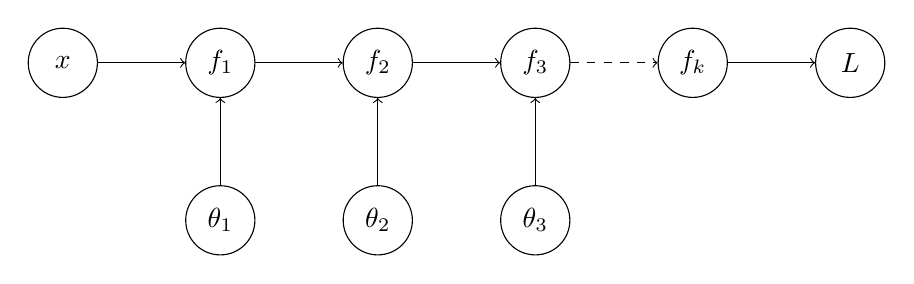
\begin{tikzpicture}[x=2cm, y=2cm]
                    \node[state] (x) at (0, 0) {$x$};
                    \node[state] (f1) at (1, 0) {$f_1$};
                    \node[state] (f2) at (2, 0) {$f_2$};
                    \node[state] (f3) at (3, 0) {$f_3$};
                    \node[state] (fk) at (4, 0) {$f_k$};
                    \node[state] (l) at (5, 0) {$L$};
                    \node[state] (t1) at (1, -1) {$\theta_1$};
                    \node[state] (t2) at (2, -1) {$\theta_2$};
                    \node[state] (t3) at (3, -1) {$\theta_3$};

                    \draw
                    (x) edge[->] (f1)
                    (f1) edge[->] (f2)
                    (f2) edge[->] (f3)
                    (f3) edge[->, dashed] (fk)
                    (fk) edge[->] (l)
                    (t1) edge[->] (f1)
                    (t2) edge[->] (f2)
                    (t3) edge[->] (f3);
                \end{tikzpicture}
            \end{center}
            If we want to learn in this model, we need to take derivatives with respect to all parameters we've defined ($\mat{A}$ and $\vec{b}$ in each layer).
            However, the former is a matrix; hence we need to take the derivative of a function with respect to a matrix, such as (note that this is no longer matrix multiplication, even if they both look like matrices; will be explained later);
            $$\dif{}{\theta} \vec{x}^\top \mat{A}(\theta) \vec{x} \text{ or } \dif{}{\mat{A}} || \mat{A}\vec{x} - \vec{y} ||^2$$
            When taking the derivative of a vector with respect to a vector, we had two indices which could be nicely represented in a matrix.
            But in the case of differentiating with respect to a matrix, we have the indices of the vector, as well as a grid of indices in the matrix.
            \medskip

            Functions of matrices are no different to functions of vectors; they're still just functions of many different numbers - hence a function of a matrix $\mat{A} \in \mathbb{R}^{M \times N}$ remains a multivariate function.
            \begin{align*}
                f(\mat{A}) & = || \mat{A}\vec{x} - \vec{y} ||^2 \\
                f(A_{1, 1}, A_{2, 1}, \dots, A_{M, 1}, \dots, A_{M, N}) & = \summation{i}{} \left(\summation{i,j}{} A_{i, j} x_j - y_i\right)
            \end{align*}
            The chain rule remains the same; where we compute all the partial derivatives with respect to the elements;
            \begin{align*}
                f(\vec{g}) = || \vec{g} ||^2 \\
                \vec{g}(\mat{A}) & = \mat{A}\vec{x} - \vec{y} \\
                \pdif{f}{A_{i, j}} & = \summation{k}{} \pdif{f}{g_k} \pdif{g_k}{A_{i, j}}
            \end{align*}
            Another example;
            \begin{align*}
                f(\mat{A}) & = \vec{x}^\top\mat{A}\vec{x} \\
                \pdif{f}{\theta} & = \summation{j,k}{} \pdif{f}{A_{j, k}} \pdif{A_{j, k}}{\theta}
            \end{align*}
            The difficulty lies in defining the notation that uses well-defined mathematical operations.
            The chain rule worked well before as we had a nice multiplication in the form of matrix multiplication; this is no longer the case here (see the note prior).
            Recall the previous notation;
            $$\dif{f}{\theta} = \dif{f}{\mat{A}} \dif{\mat{A}}{\theta} \text{ and } \dif{f}{\mat{A}} = \dif{f}{\vec{g}} \dif{\vec{g}}{\mat{A}}$$
            A derivative of a vector with respect to a matrix is a rank 3 tensor (a vector can be seen as a rank 1 tensor, and a matrix as rank 2).
            This representation with higher-dimensional tensors generalises well.
            Recall that a function $\vec{f} : \mathbb{R}^N \to \mathbb{R}^M$ ($M$ target dimensions and $N$ input dimensions) has the following;
            $$\dif{\vec{f}}{\vec{x}} \in \mathbb{R}^{M \times N}\text{,\ \ \ \ } \mathrm{d}\vec{f}[m, n] = \pdif{f_m}{x_n}$$
            This generalises when the sizes of the inputs are matrices instead, for example $\mat{f} : \mathbb{R}^{M \times N} \to \mathbb{R}^{P \times Q}$, where the gradient is a tensor;
            $$\dif{\mat{f}}{\mat{X}} \in \mathbb{R}^{M \times N}\text{,\ \ \ \ } \mathrm{d}\mat{f}[p, q, m, n] = \pdif{f_{p, q}}{X_{m, n}}$$
            Applying the chain rule to a particular matrix valued function - take the example of $f \in \mathbb{R}$ being a scalar function of $\mat{A} \in \mathbb{R}^{(P \times Q) \times (N \times M)}$, which is a function of $\vec{\theta} \in \mathbb{R}^L$;
            \setcounter{equation}{0}
            \begin{align}
                \underbrace{\dif{f}{\vec{\theta}}}_{1 \times L} & = \underbrace{\dif{f}{\mat{A}}}_{1 \times (N \times M)} \underbrace{\dif{\mat{A}}{\vec{\theta}}}_{(N \times M) \times L} \\
                & = \dif{f}{\mathrm{vec}\vec{A}} \cdot \dif{\mathrm{vec}\vec{A}}{\vec{\theta}} \\
                \mathrm{vec}\begin{bmatrix}
                    a & b \\
                    c & d
                \end{bmatrix} & = \begin{bmatrix}
                    a \\ c \\ b \\ d
                \end{bmatrix}
            \end{align}
            \begin{enumerate}[(1)]
                \itemsep0em
                \item the issue is that we end up with a tensor $\mathbb{R}^{(N \times M) \times L}$
                \item we're now back to doing differentiating with vectors, leading to matrix multiplication
                \item note that changing a matrix into a vector gives a column vector of the matrix by columns
            \end{enumerate}
            Automatic differentiation packages keep track of all these axes in these higher order tensors which contain these derivatives and figure out which axes to sum over by looking at the input shape of the function $f : \mathbb{R}^{N \times M} \to \mathbb{R}$, consistent with the matrix valued chain rule.
            The most unambiguous way to deal with this is to write it all as a vector, leading to matrix multiplication.
            \subsubsection*{Example of Multivariate Function}
                The function is $f : \mbbr^{N \times M} \to \mbbr^N$, defined as;
                \begin{align*}
                    \vec{f} & = \underbrace{\mat{A}}_{N \times M} \underbrace{\vec{x}}_{M \times 1} \\
                    \dif{\vec{f}}{\mat{A}} & \in \mbbr^{N \times (N \times M)} \\
                    \pdif{f_i}{A_{j, k}} & = \pdif{}{A_{j, k}} \left(\summation{m}{} A_{i, m} x_m\right) \\
                    & = \summation{m}{} \pdif{A_{i, m}}{A_{j, k}}x_m \\
                    & = \summation{m}{}\delta_{nj} \delta_{mk} x_m \\
                    & = \delta_{ij} x_k
                \end{align*}
                This gives the following three-dimensional tensor, taking the convention of putting the outputs ($i$) along the column.
                Note that there are zeroes everywhere, other than the \violet{leading diagonal} on $i,j$ where the elements of $\vec{x}$ are.
                \begin{center}
                    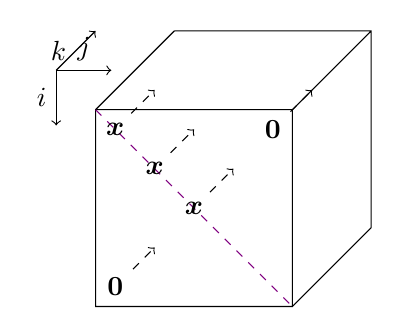
\begin{tikzpicture}[x=0.5cm, y=0.5cm]
                        \draw
                        (0, 0) -- (5, 0) -- (5, -5) -- (0, -5) -- cycle
                        (2, 2) -- (7, 2) -- (7, -3)
                        (0, 0) -- (2, 2)
                        (5, 0) -- (7, 2)
                        (5, -5) -- (7, -3);

                        \begin{scope}
                            \draw
                            (-1, 1) edge[->, left] node{$k$} (0, 2)
                            (-1, 1) edge[->, above] node{$j$} (0.4, 1)
                            (-1, 1) edge[->, left] node{$i$} (-1, -0.4);
                        \end{scope}

                        \draw[violet] (0, 0) edge[dashed] (5, -5);
                        \node (bl) at (0.5, -4.5) {$\vec{0}$};
                        \node (tr) at (4.5, -0.5) {$\vec{0}$};
                        \node (x1) at (0.5, -0.5) {$\vec{x}$};
                        \node (x2) at (1.5, -1.5) {$\vec{x}$};
                        \node (x3) at (2.5, -2.5) {$\vec{x}$};
                        \draw
                        (x1) edge[->, dashed] ($(x1) + (1, 1)$)
                        (x2) edge[->, dashed] ($(x2) + (1, 1)$)
                        (x3) edge[->, dashed] ($(x3) + (1, 1)$)
                        (bl) edge[->, dashed] ($(bl) + (1, 1)$)
                        (tr) edge[->, dashed] ($(tr) + (1, 1)$);
                    \end{tikzpicture}
                \end{center}
            \subsubsection*{Backpropagation}
                Recall that a neural network is essentially a stack of function estimators, such that the output of a previous function becomes the input of the next function.
                The loss function is typically something with respect to an error producing output (observed value $y_i$ compared to some computed value $f_i$).
                As such, $L$ is a function of all the parameters that make up the network; $L(\mat{A_1}, \vec{b_1}, \mat{A_2}, \vec{b_2}, \dots)$, which can also be written with $\vec{\theta}$ parameters.
                Consider the following example of a single-layer network;
                \begin{center}
                    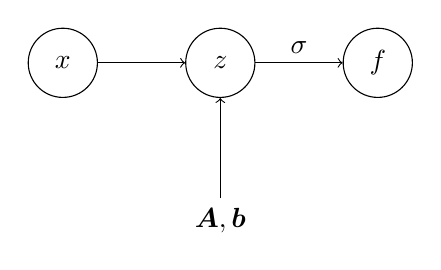
\begin{tikzpicture}[x=2cm, y=2cm]
                        \node[state] (x) at (0, 0) {$x$};
                        \node[state] (z) at (1, 0) {$z$};
                        \node[state] (f) at (2, 0) {$f$};
                        \node (ab) at (1, -1) {$\mat{A}, \vec{b}$};

                        \draw
                        (x) edge[->] (z)
                        (z) edge[->, above] node{$\sigma$} (f)
                        (ab) edge[->] (z);
                    \end{tikzpicture}
                \end{center}
                In this example, let $\sigma$ (activation function) be $\tanh$ applied to some linear transformation (which we can denote $\vec{z}$), with $\vec{z} \in \mbbr^M, \vec{x} \in \mbbr^N, \mat{A} \in \mbbr^{M \times N}, \vec{b} \in \mbbr^M$.
                Also note that we have a loss function, $L$;
                \begin{align*}
                    \vec{\theta} & = \{\mat{A}, \vec{b}\} \\
                    L(\vec{\theta}) & = \frac{1}{2} || \vec{e} ||^2 \\
                    \vec{e} & = \vec{y} - \vec{f}_{\vec{\theta}}(\vec{x}) \\
                    \vec{f} & = \tanh(\underbrace{\mat{A}\vec{x} + \vec{b}}_{\vec{z}}) \\
                    \underbrace{\pdif{L}{\vec{e}}}_{1 \times M} & = \vec{e}^\top \\
                    \underbrace{\pdif{\vec{e}}{\vec{f}}}_{M \times M} & = -\mat{I} \\
                    \underbrace{\pdif{\vec{f}}{\vec{b}}}_{M \times M} & = \underbrace{\pdif{\vec{f}}{\vec{z}}}_{M \times M} \underbrace{\pdif{\vec{z}}{\vec{b}}}_{M \times M} \\
                    \underbrace{\pdif{\vec{f}}{\mat{A}}}_{M \times (M \times N)} & = \underbrace{\pdif{\vec{f}}{\vec{z}}}_{M \times M} \underbrace{\pdif{\vec{z}}{\mat{b}}}_{M \times (M \times N)} \\
                    \pdif{\vec{f}}{\vec{z}} & = \diag(1 - \tanh^2(\vec{z})) \\
                    \pdif{\vec{z}}{\vec{b}} & = \mat{I} \\
                    \pdif{\vec{z}}{\mat{A}} & = \begin{bmatrix}
                        \vec{x}^\top & \cdots & \vec{0}^\top & \cdots & \vec{0}^\top \\
                        \vdots & \ddots & \vdots & \ddots & \vdots \\
                        \vec{0}^\top & \cdots & \vec{x}^\top & \cdots & \vec{0}^\top \\
                        \vdots & \ddots & \vdots & \ddots & \vdots \\
                        \vec{0}^\top & \cdots & \vec{0}^\top & \cdots & \vec{x}^\top
                    \end{bmatrix}
                \end{align*}
                If we blindly applied the rules we know, we'd be able to solve it with many computations of partial derivatives.
                The idea behind backpropagation is to find an order of computing partial derivatives that maximally reuses what we've computed.
                Consider the following;
                $$L(\vec{\theta_1}, \vec{\theta_2}, \dots, \vec{\theta_K}) = || \vec{y} - \vec{f_{\vec{\theta_K}}}(\vec{f_{\vec{\theta_{K - 1}}}}(\dots \vec{f_{\vec{\theta_2}}}(\vec{f_{\vec{\theta_1}}}(\vec{x})) \dots))||^2$$
                This has the following relation (anything that hasn't been previously computed is in \violet{violet});
                \begin{align*}
                    \pdif{L}{\vec{\theta_K}} & = \violet{\pdif{L}{\vec{f_K}} \pdif{\vec{f_K}}{\vec{\theta_K}}} \\
                    \pdif{L}{\vec{\theta_{K - 1}}} & = \pdif{L}{\vec{f_K}} \violet{\pdif{\vec{f_K}}{\vec{f_{K - 1}}} \pdif{\vec{f_{K - 1}}}{\vec{\theta_{K - 1}}}} \\
                    \pdif{L}{\vec{\theta_{K - 2}}} & = \pdif{L}{\vec{f_K}} \pdif{\vec{f_K}}{\vec{f_{K - 1}}} \violet{\pdif{\vec{f_{K - 1}}}{\vec{f_{K - 2}}} \pdif{\vec{f_{K - 2}}}{\vec{\theta_{K - 2}}}} \\
                    \pdif{L}{\vec{\theta_{K - 3}}} & = \pdif{L}{\vec{f_K}} \pdif{\vec{f_K}}{\vec{f_{K - 1}}} \pdif{\vec{f_{K - 1}}}{\vec{f_{K - 2}}} \violet{\pdif{\vec{f_{K - 2}}}{\vec{f_{K - 3}}} \pdif{\vec{f_{K - 3}}}{\vec{\theta_{K - 3}}}} \\
                    \pdif{L}{\vec{\theta_i}} & = \pdif{L}{\vec{f_K}} \pdif{\vec{f_K}}{\vec{f_{K - 1}}} \cdots \violet{\pdif{\vec{f_{i + 1}}}{\vec{f_i}} \pdif{\vec{f_i}}{\vec{\theta_i}}}
                \end{align*}
                All the partial gradients that are carried around are vectors, being significantly more computationally efficient than matrices.
        \subsection*{Lecture 3 - Probability and Statistics}
            \subsubsection*{Overfitting}
                Recall the curve fitting problem was to find to find a curve that predicts well for unseen inputs, by minimising the loss on the training points.
                The idea is that it needs to fit the training data well, to fit for unseen data.
                $$L(\vec{\theta}) = \summation{n}{} (f(\vec{x}_n; \vec{\theta}) - y_n)^2$$
                Consider how many basis functions we should use (considering polynomial);
                $$q \in 0, \dots, Q: \vec{\phi}(x) = \begin{bmatrix}
                    1 & \cdots & x^q
                \end{bmatrix}^\top$$
                For each order we add, we have a more `wiggly' function that approaches our training data.
                However, as we get closer to the training data, our predictions further away from our training points start to become more erratic.
                $$f_M(\vec{x}_n; \vec{\theta}) = \summation{m = 0}{M} x^m \theta_m$$
                For models $M_1 \leq M_2$, the model $M_2$ can represent all functions that $M_1$ can - therefore increasing the order can never worsen the fit on the training data.
                Closed-form optimisation will find the exact minimum, hence (the training loss will always get smaller when we add basis functions);
                $$\min_{\vec{\theta}}L_{M_2}(\vec{\theta}) \leq \min_{\vec{\theta}}L_{M_1}(\vec{\theta})$$
                Typical practice is to split data into a training and a test set.
                The training set is actually used to find the parameters of a model and the test data shows how well the data predicts on unseen data.
                We can estimate some loss on the training set, using argmin (which finds the argument that minimises a function);
                $$\vec{\theta^*} = \argmin_{\vec{\theta}}L(\vec{\theta})$$
                $$L_\text{test} = \frac{1}{N_\text{test}}(f(x_n; \vec{\theta^*}) - y_n)^2$$
                The training error should decrease with higher polynomial degrees, whereas the test error should also decrease until a certain point, when it starts to increase (overfitting).
            \subsubsection*{Probability Theory}
                We need to formalise this as follows;
                \begin{itemize}
                    \itemsep0em
                    \item $\Omega$ \hfill set of all possible outcomes
                        \subitem for a die; $\Omega = \{1, 2, 3, 4, 5, 6\}$
                    \item $E = \{\omega_i \in \Omega\}_{i = 1}^I$ \hfill event is a set of outcomes
                        \subitem for an event that states the value of the die is greater than 3; $E = \{4, 5, 6\}$
                    \item $\mathcal{A}$ \hfill set of all events (a set of sets)
                    \item $X, Y$ \hfill random variables (functions on outcomes to the target set $\tau$, simplifies event structure)
                        $$X: \Omega \to \tau$$
                \end{itemize}
                Consider $\Omega$ to be all possible outcomes of a presidential election (can have varying granularity).
                This could be from the level of what each person voted, and so on.
                $X(\omega)$ is a simple binary outcome, whether person $X$ is president or not (1 or 0, respectively).
                \medskip

                For the scenario of flipping two coins, $\Omega = \{HT, TH, HH, TT\}$.
                Let $X(\omega)$ be the number of heads;
                $$X(\omega) = \begin{cases}
                    0 & TT \\
                    1 & HT, TH \\
                    2 & HH
                \end{cases}$$
                A probability measure is a function on sets with the following properties;
                \begin{itemize}
                    \itemsep0em
                    \item maps from a particular element in the set of all possible events to a real value, larger than $0$
                        $$P : \mathcal{A} \to \mbbr, P(E) \geq 0$$
                    \item probability of the set of outcomes is equal to 1 (something always happens)
                        $$P(\Omega) = 1$$
                    \item union of events is the sum when there is no intersection % see recording
                        $$P\left(\bigcup\limits_{i = 1}{\infty} E_i\right) = \summation{i}{} P(E_i) \text{ when } E_i \cap E_j = \emptyset\ \forall i, j, i \neq j$$
                \end{itemize}
                These axioms describe the reasoning about frequencies of recurring events and the plausibility of beliefs.
                Our goal is to compute probabilities on the outcomes of random variables (all possible outcomes of $\Omega$ such that $X(\omega)$ is in $S$ - what is the set of all outcomes that would give the random variable values that we care about);
                $$P_X(S) = P(X \in S) = P(X^{-1}(S)) = P(\{\omega \in \Omega : X(\omega) \in S\})$$
                We can also have multiple random variables as an outcome of the same event.
                Using the concrete example of the presidential election;
                \begin{align*}
                    X(\omega) & = \begin{cases}
                        1 & \text{person $X$ wins} \\
                        0 & \text{otherwise}
                    \end{cases} \\
                    Y(\omega) & = \begin{cases}
                        1 & \text{person $X$ wins Arkansas} \\
                        0 & \text{otherwise}
                    \end{cases}
                \end{align*}
                Similarly, we can ask probabilities on the pairs, with the same intuition;
                $$P_{X, Y}(S) = P((X, Y) \in S) = P(\{\omega \in \Omega : (X(\omega), Y(\omega)) \in S\})$$
                We might want to compute the probability of an event happening for a random variable.
                For a finite target set, we just need to specify the probability of each of these outcomes ($\frac{1}{6}$ for each die face).
                Note that for a single event, common notation could be $P(X = x) = p_X(x)$, or even lazier $p(x)$ (with the $x$ implying a random variable $X$).
                Similar notation can be used for multiple random variables; $P(X = x, Y = y) = P_{X, Y}(x, y) = P(x, y)$.
                In the discrete case, probabilities juts need to be specified for each pair.
                \medskip

                If we have the probabilities of multiple random variables, we can use this to find the probability of just one of the RVs.
                This is marginal probability.
                For example, if we have $p_{X, Y}(x, y)$ and we just want $p(x)$;
                \begin{align*}
                    P(X = x) & = P((X, Y) \in \{((x, y) : y \in \tau_Y)\}) \\
                    & = \summation{y \in \tau_Y}{} p_{X, Y}(x, y)
                \end{align*}
                An example of this is from \textit{MacKay}; looking at a certain row of the joint table and normalise the occurrences on the same row to sum to 1.
                Conditional probability is as follows;
                \begin{align*}
                    P(X = x\ |\ Y = y) & = \frac{P(X = x, Y = y)}{\summation{x^\prime}{} P(X = x^\prime, Y = y)}\\
                    & = \frac{P(X = x, Y = y)}{P(Y = y)} \\
                    P(A\ |\ B) & = \frac{P(A \cap B)}{P(B)}
                \end{align*}
                The two rules are as follows (and Bayes' rule can be derived);
                \begin{itemize}
                    \itemsep0em
                    \item sum rule \hfill $p(x) = \summation{y}{} p(x, y)$
                    \item product rule \hfill $p(x, y) = p(y\ |\ x)p(x) = p(y)p(x\ |\ y)$
                    \item Bayes' rule \hfill $p(y\ |\ x) = \frac{p(x\ |\ y)p(y)}{p(x)}$
                \end{itemize}
                Statistical independence states that two events are independent if $P(A \cap B) = P(A)P(B)$ or $P(A\ |\ B) = P(A)$ - or $A$ doesn't depend on $B$.
                Two random variables are independent if $p(X = x, Y = y) = p(x)p(y)$, also written as $X \independent Y$.
                \medskip

                However, when it's a continuous random variable, the probability of any particular outcome is zero.
                This is the case where we have $X : \Omega \to \mbbr$
                However, it's more meaningful to ask $P(a \leq X \leq b)$, which can be specified as follows;
                $$P(a \leq X \leq b) = \defint{a}{b}{f_X(x)}{x} = \defint{a}{b}{p(x)}{x}$$
                And similarly for multiple random variables;
                $$P(a \leq X \leq b, c \leq Y \leq d) = \defint{a}{b}{\defint{c}{d}{f_{X, Y}(x, y)}{y}}{x}$$
                The rules are similar;
                \begin{itemize}
                    \itemsep0em
                    \item sum rule \hfill $p(x) = \int_y p(x, y) \mathrm{d}y$
                    \item product and Bayes' rule are exactly the same (note we are using the shorthand $f_X(x) = p(x)$ when $x \in \mbbr$)
                \end{itemize}
                The general form of a \textbf{moment} is as follows;
                $$\mathbb{E}_X[g(X)] = \indefint{p(x)g(x)}{x}$$
                For a distribution over a vector, the mean vector works similar to the partial derivatives from before (note $\vec{a}$ is just any `direction');
                \begin{align*}
                    p(\vec{x}) & = p(x_1, x_2, \dots) \\
                    \mathbb{E}_{\vec{X}}[\vec{a}^\top\vec{x}] & = \indefint{\vec{a}^\top\vec{x}p(\vec{x})}{\vec{x}} \\
                    & = \indefint{\summation{i}{} a_i x_i p(\vec{x})}{\vec{x}} \\
                    & = \summation{i}{} a_i \indefint{x_i p(\vec{x})}{\vec{x}} \\
                    & = \summation{i}{} a_i \indefint{x_i p(x_i) p(\{x_j\}_{i \neq j}\ |\ x_i)}{\vec{x}} \\
                    & = \summation{i}{} a_i \indefint{x_i p(x_i)}{x_i} \underbrace{\indefint{p(\{x_j\}_{i \neq j}\ |\ x_i)}{\{x\}}}_{= 1} \\
                    & = \vec{a}^\top\vec{\bar{x}}
                \end{align*}
                A similar approach can be taken for variance;
                \begin{align*}
                    \mathbb{V}_{\vec{X}}[\vec{a}^\top\vec{x}] & = \indefint{(\vec{a}^\top\vec{x} - \vec{a}^\top\vec{\bar{x}})p(\vec{x})}(\vec{x}) \\
                    & = \indefint{\left(\summation{i}{} a_ix_i - a_i-\bar{x}_i\right)\left(\summation{j}{} a_jx_j - a_j-\bar{x}_j\right)p(\vec{x})}{\vec{x}} \\
                    & = \summation{i}{} \summation{j}{} a_i a_j \indefint{(x_i - \bar{x}_i)(x_j - \bar{x}_j)p(x_i, x_j)}{\{x_i, x_j\}} \\
                    & = \vec{x}^\top\mat{\Sigma}{\vec{a}}
                \end{align*}
                The intuition for the direction, for variance, is that we look at the variance in the scalar random variables along a given direction.
        \subsection*{Lecture 4 - Cross-validation}
            We can prevent overfitting by choosing a model (polynomial degree) which isn't too flexible.
            Generalisation loss represents how well our model performs in future predictions.
            The setting is that we train the model and deploy it for future predictions, making infinite predictions (limit of $N \to \infty$) in the future.
            We also incur a penalty for errors (loss function $\ell$).
            $$L_\text{test} = \limit{N}{\infty} \frac{1}{N} \summation{n = 1}{N} \ell(f(\vec{x_n}; \vec{\theta^*}), y_n)$$
            We assume the pairs $(\vec{x_n}, y_n)$ come from the \textbf{same distribution} (both training and future data), hence $\vec{x_n}, y_n \sim p(\vec{x}, y)$.
            By the law of large numbers (generalisation error) - note that this is a moment of $p(\vec{x}, y)$;
            $$L_\text{test} = \mathbb{E}_{p(\vec{x}, y)}[\ell(f(\vec{x}; \vec{\theta^*}), y)]$$
            Our goal is to estimate this loss without knowing the true joint distribution.
            We can get samples from $p(\vec{x}, y)$, and construct an estimator for $L_\text{test}$ from these samples;
            $$\hat{L}_\text{test} = \frac{1}{N_\text{test}} \summation{n = 1}{N} \ell(f(\vec{x_n}; \vec{\theta^*}), y_n)$$
            We are writing this without knowing what the density function is, just saying that it exists.
            As the number of testing points goes to infinity, the estimate approaches the true test loss.
            \medskip

            Good ML practice splits data into a training set and a test set, both of which are iid samples from this distribution.
            Only on the training set do we \textbf{minimise} the loss.
            And loss is \textbf{measured} on the test set.
            As long as \textbf{no decisions} are based on the test set, $\hat{L}_\text{test}$ will be an unbiased estimate of the true average loss.
            This loss tells us what the error would've been on particular model.
            Unbiased means;
            $$\mathbb{E}_{p(\vec{x_1}, \vec{x_2}, \dots, y_1, y_2, \dots)}[\hat{L}_\text{test}(\vec{x_1}, \vec{x_2}, \dots, y_1, y_2, \dots)] = L_\text{test}$$
            We can analyse the variance of this estimator.
            As the test set becomes larger, the variance decreases.
            $$\mathbb{V}_{\Pi_n p(\vec{x_n}, y_n)} \left[\frac{1}{N} \summation{n = 1}{N} \ell(f(\vec{x_n}; \vec{\theta^*}), y_n)\right] = \frac{1}{N} \mathbb{V}_{p(\vec{x}, \vec{y})}[\ell(f(\vec{x_n}; \vec{\theta^*}), y)]$$
            If we have a small variance, the error of the estimator is smaller.
            Chebyshev's inequality states that the probability of a variable being far away (more than $k$ times the standard deviation) from the mean (the true value we want);
            $$P(| X - \bar{X} | \geq k\sigma) \geq \frac{1}{k^2}$$
            We want to evaluation a collection of models (different orders of polynomials) on the test set and then pick the model with the lowest test loss.
            However, we may want to ask whether this is still an unbiased estimate of the test loss.
            Note that $\vec{\theta^*}$ is now a function of the test set, therefore the estimator is no longer unbiased - therefore we cannot use the test set to select the model if we want an accurate estimate of the test loss;
            $$\mathbb{E}_{\Pi_n p(\vec{x_n}, y_n)} \left[\frac{1}{N} \summation{n = 1}{N} \ell(f(\vec{x_n}; \vec{\theta^*}(\{\vec{x_i}, y_i\}_{i = 1}^N)), y_n)\right] \neq \mathbb{E}_{p(\vec{x}, \vec{y})}[\ell(f(\vec{x_n}; \vec{\theta^*}), y)]$$
            All labelled data is split into training data and test data.
            The training data is split further to a training set (to find the parameters of the model) and a validation set (to select the model).
            Once we've select the model based on the validation set, we can use the true test set (kept completely separate) to find an unbiased estimator.
            However, with a small validation set there would be large variance (possibly choosing wrong model), whereas a large validation set would lead to smaller training sets, hence wrong parameters could be chosen.
            \medskip

            Cross-validation splits the data into training and validation sets in multiple ways, and computes the validation performance for each split.
            The average of these values is the cross-validation loss (no longer unbiased, however small).
            \begin{enumerate}
                \itemsep0em
                \item split data in $K$ different ways
                \item for each model;
                    \begin{enumerate}
                        \itemsep0em
                        \item for each split
                            \begin{enumerate}
                                \itemsep0em
                                \item find parameters of model
                                \item compute loss on validation set
                            \end{enumerate}
                        \item calculate average validation loss for all splits
                    \end{enumerate}
                \item pick model with lowest cross-validation loss
            \end{enumerate}
        \subsection*{Lecture 5 - Gradient Descent}
            An optimisation is can be formulated as an objective function $L : \mbbr^D \to \mbbr$ (parameter space to scalar) which roughly tells us how well the model performs on the training data, with an unconstrained minimisation (search parameter in the full space);
            $$\vec{\theta^*} = \argmin_{\vec{\theta}} L(\vec{\theta})$$
            Gradient-based optimisation is a class of methods which perform the following steps;
            \begin{itemize}
                \itemsep0em
                \item pick starting point $\vec{\theta_0}$
                \item iterative update the parameters to give a sequence $\vec{\theta_1}, \dots, \vec{\theta_T}$
                \item choose the update by computing the gradient $\nabla_{\vec\theta}L(\vec{\theta_t})$
                \item repeat until we reach a stopping criterion (such as computation budget or gradient size)
            \end{itemize}
            The gradient descent algorithm is as follows, with a starting point $\vec{\theta_0}$ and a sequence of step sizes $\gamma_t$;
            \begin{enumerate}[1.]
                \itemsep0em
                \item set $\vec{\theta_{t + 1}} = \vec{\theta_t} - \gamma_t \nabla_{\vec{\theta}}L(\vec{\theta_t})$
                \item repeat the first step until the stopping criterion is met
            \end{enumerate}
            Consider the following model (note the use of matrices), our goal is to find $\mat{\theta} \in \mbbr^{D \times 1}$, such that $\mat{y} \approx \mat{X}\mat{\theta}$;
            \begin{align*}
                \mathcal{D} & = \{ \mat{X}, \mat{y} \} & \text{dataset} \\
                \mat{X} & = \begin{bmatrix}
                    \vec{x_1} & \cdots & \vec{x_N}
                \end{bmatrix}^\top & \in \mbbr^{N \times D} \\
                \mat{y} & = \begin{bmatrix}
                    y_1 & \cdots & y_N
                \end{bmatrix}^\top & \in \mbbr^{N \times 1} \\
                \mat{X}^\top & = \begin{bmatrix}
                    \uparrow & \uparrow & & \uparrow \\
                    \vec{x_1} & \vec{x_2} & \cdots & \vec{x_N} \\
                    \downarrow & \downarrow & & \downarrow \\
                    1 & 1 & & 1
                \end{bmatrix}
            \end{align*}
            The model and loss are as follows (assume a mean of zero and some variance) and the loss is the $\ell_2$ norm.
            We are taking the gradient as the transpose of the derivative of $L$ with respect to $\vec{\theta}$ (a column vector);
            \begin{align*}
                f(\vec{x}, \vec{\theta}) & = \vec{x}^\top\vec{\theta} \\
                y & = f(\vec{x}, \vec{\theta}) + \epsilon & \epsilon \sim \mathcal{N}(0, \sigma^2) \\
                L(\vec{\theta}) & = \frac{1}{2 \sigma^2} \summation{n}{} (f(\vec{x_n}, \vec{\theta}) - y_n)^2 \\
                & = \frac{1}{2 \sigma^2} || \mat{y} - \mat{X}\mat{\theta} ||_2^2 \\
                \nabla_{\vec{\theta}} L(\vec{\theta}) & = \dif{L}{\vec{\theta}}^\top \\
                & = \frac{1}{\sigma^2} \mat{X}^\top(\mat{X}\mat{\theta} - \mat{y}) & \text{setting $= 0$, to get pseudo-inverse $\Rightarrow$} \\
                \frac{1}{\sigma^2} \mat{X}^\top\mat{X}\mat{\theta^*} & = \frac{1}{\sigma^2} \mat{X}^\top\mat{y} & \Rightarrow \\
                \mat{\theta^*} & = (\mat{X}^\top\mat{X})^{-1}\mat{X}^\top\mat{y}
            \end{align*}
            The gradient descent for linear regression can be written as follows, assuming constant step-sizes ($\gamma_t = \gamma$);
            \begin{enumerate}[1.]
                \itemsep0em
                \item define the starting point $\mat{\theta_0}$
                \item update $\mat{\theta_{t + 1}}$
                    \begin{align*}
                        \mat{\theta_{t + 1}} & = \mat{\theta_t} - \gamma_t \nabla_{\mat{\theta}}L(\vec{\theta_t}) \\
                        & = \mat{\theta_t} - \gamma\frac{1}{\sigma^2} \mat{X}^\top(\mat{X}\mat{\theta_t} - \mat{y}) \\
                        & = (\mat{I} - \frac{\gamma}{\sigma^2}\mat{X}^\top\mat{X})\mat{\theta_t} + \frac{\gamma}{\sigma^2}\mat{X}^\top\mat{y}
                    \end{align*}
                \item repeat until stopping criterion
            \end{enumerate}
            We will study the gradient descent update equation (final line).
            This forms a geometric series ($x_{t + 1} = a x_t + b$), which can be written as $\alpha^t x_0 + \beta$ (which applies to vectors as well as scalars).
            \begin{align*}
                \mat{\theta_{t + 1}} + \mat{\beta} & = \mat{A}(\mat{\theta_t} + \mat{\beta}) & \Rightarrow \\
                \mat{\theta_{t + 1}} & = \mat{A}\mat{\theta_t} + (\mat{A} - \mat{I})\mat{\beta} & \Rightarrow \\
                \mat{A} & = (\mat{I} - \frac{\gamma}{\sigma^2}\mat{X}^\top\mat{X}) \\
                (\mat{A} - \mat{I})\mat{\beta} & = \frac{\gamma}{\sigma^2}\mat{X}^\top\mat{y} & \Rightarrow \\
                -\frac{\gamma}{\sigma^2}\mat{X}^\top\mat{X}\mat{\beta} & = \frac{\gamma}{\sigma^2}\mat{X}^\top\mat{y} & \Rightarrow \\
                \mat{\beta} & = -(\mat{X}^\top\mat{X})^{-1}\mat{X}^\top\mat{y} \\
                & = -\mat{\theta^*}
            \end{align*}
            This iterative update gives the following result;
            $$\mat{\theta_t} = (\mat{I} - \frac{\gamma}{\sigma^2}\mat{X}^\top\mat{X})^t(\mat{\theta_0} - \mat{\theta^*}) + \mat{\theta^*}$$
            Note that this tells us the gradient descent converges (as $t$ gets larger) $\mat{\theta_t} \to \mat{\theta^*}$ if;
            $$(\mat{I} - \frac{\gamma}{\sigma^2}\mat{X}^\top\mat{X})^t(\mat{\theta_0} - \mat{\theta^*}) \to \mat{0}$$
            In an $\mbbr^D$ space, the space can be constructed by a span of basis vectors.
            For example, $\mbbr^2 = \mathrm{span}(\{\vec{e_1}, \vec{e_2}\})$ and $\vec{e_i} \perp \vec{e_j}, || \vec{e_i} || = 1$.
            Any vector in this space can be written as a linear combination of the basis vectors.
            For the standard basis, assume 2-dimensions, $\vec{x} = (x_1, x_2)^\top$, then $\vec{x}^\top\vec{e_i} = x_i$.
            \medskip

            A left multiply of $\mat{Q}^{-1}$ on $\vec{x}$ is known as a change of basis from $\{\vec{e_1}, \vec{e_2}\}$ to $\{\vec{q_1}, \vec{q_2}\}$;
            \begin{align*}
                \mat{Q} & = \begin{bmatrix}
                    q_{1,1} & q_{1,2} \\
                    q_{2,1} & q_{2,2}
                \end{bmatrix} \\
                & = \begin{bmatrix}
                    \vec{q_1} & \vec{q_2}
                \end{bmatrix} \\
                \mat{Q}^{-1} & = \begin{bmatrix}
                    q_{1,1} & q_{2,1} \\
                    q_{1,2} & q_{2,2}
                \end{bmatrix} \\
                & = \begin{bmatrix}
                    \vec{q_1}^\top \\ \vec{q_2}^\top
                \end{bmatrix} \\
                \vec{z} & = \mat{Q}^{-1}\vec{x} \\
                z_1 & = \vec{q_1}^\top\vec{x} \\
                z_2 & = \vec{q_2}^\top\vec{x}
            \end{align*}
            If we were to stretch this vector in the $\mat{Q}$ basis;
            \begin{align*}
                \vec{z^\prime} & = \mat{\Lambda}\mat{Q}^{-1}\vec{x} \\
                z_1^\prime & = \lambda_1\vec{q_1}^\top\vec{x} \\
                z_2^\prime & = \lambda_2\vec{q_2}^\top\vec{x} \\
                \mat{\Lambda} & = \begin{bmatrix}
                    \lambda_1 & 0 \\
                    0 & \lambda_2
                \end{bmatrix}
            \end{align*}
            To return to the canonical basis, after stretching by $\mat{\Lambda}$ in the $\mat{Q}$ basis, we have $\vec{x^\prime} = \mat{Q} \mat{\Lambda} \mat{Q}^{-1} \vec{x}$.
            Consider the case where we have $\vec{x^\prime} = \mat{A}\vec{x}$, for some $\mat{A} \in \mbbr^{D \times D}$.
            We want to find $\mat{A} = \mat{Q} \mat{\Lambda} \mat{Q}^{-1}$.
            The goal is to find scalar $\lambda$ (eigenvalue) and vector (eigenvector) $\vec{q}$ such that $\mat{A}\vec{q} = \lambda\vec{q}$, if solutions exist for this, we have $\mat{A} = \mat{Q} \mat{\Lambda} \mat{Q}^{-1}$ where $\mat{\Lambda} = \mathrm{diag}(\lambda_1, \dots, \lambda_D)$.
            If $\mat{A}$ is symmetric, there will be $D$ pairs of solutions of eigenvectors and eigenvalues, such that the column vectors ($\mat{Q} = (\vec{q_1}, \dots, \vec{q_D})$) form an orthonormal basis (such that $\mat{Q}^{-1} = \mat{Q}^\top$) and $\lambda_1 \geq \lambda_2 \geq \cdots \geq \lambda_D$.
            Additionally, if $\mat{A}$ is positive semi-definite, then $\lambda_D \geq 0$.
            To find this, we first assume $\vec{q} \neq \vec{0}$.
            By $\mat{A}\vec{q} = \lambda\vec{q}$, we can get $(\mat{A} - \lambda\mat{I})\vec{q} = \vec{0}$.
            With the assumption, we find $\lambda$ such that $\det(\mat{A} - \lambda\mat{I}) = 0$ - once we have this, it can be plugged in and solved to obtain $\vec{q}$.
            \medskip

            The determinant tells us how the volume is scaled by linear transformation.
            If the determinant is zero ($\det(\mat{A} - \lambda\mat{I}) = 0$), then some subspace in $\mbbr^D$ is collapsed into a line $\{ \vec{0} \}$, implying that there is some $\vec{q} \neq 0$ such that $(\mat{A} - \lambda\mat{I}) \vec{q} = \vec{0}$.
            If $\lambda$ is an eigenvalue of $\mat{A}$, then $\lambda^t$ is an eigenvalue of $\mat{A}^t$.
            Additionally, $\lambda + \alpha$ is an eigenvalue of $\mat{A} + \alpha\mat{I}$;
            $$\mat{A} + \alpha\mat{I} = \mat{Q}\mat{\Lambda}\mat{Q}^{-1} + \mat{Q}\alpha\mat{I}\mat{Q}^{-1} = \mat{Q}(\mat{\Lambda} + \alpha\mat{I})\mat{Q}^{-1} \Rightarrow \mat{\Lambda} + \alpha\mat{I} = \mathrm{diag}(\lambda_1 + \alpha, \dots, \lambda_D + \alpha)$$
            By combining these, if $\lambda$ is an eigenvalue of $\mat{A}$, then it follows that $(\lambda + \alpha)^t$ is an eigenvalue of $(\mat{A} + \alpha\mat{I})^t$.
            Note that the corresponding eigenvector in the pair doesn't change.
            \medskip

            The Rayleigh quotient is bounded by the eigenvalues of $\mat{A}$ (assuming symmetric);
            $$\lambda_\text{min}(\mat{A}) \leq \underbrace{R(\mat{A}, \vec{x}) = \frac{\vec{x}^\top\mat{A}\vec{x}}{|| \vec{x} ||_2^2} = \frac{\vec{x}^\top\mat{A}\vec{x}}{\vec{x}^\top\vec{x}}}_\text{Rayleigh quotient} \leq \lambda_\text{max}(\mat{A}) \Rightarrow \lambda_\text{min}(\mat{A})|| \vec{x} ||_2^2 \leq \vec{x}^\top\mat{A}\vec{x} \leq \lambda_\text{max}(\mat{A})|| \vec{x} ||_2^2$$
            This result comes from the following;
            \begin{align*}
                \vec{x}^\top\mat{A}\vec{x} & = \vec{x}^\top\mat{Q}\mat{\Lambda}\underbrace{\mat{Q}^\top\vec{x}}_{\vec{z}} \\
                & = \vec{z}^\top\mat{\Lambda}\vec{z} \\
                \vec{x}^\top\vec{x} & = \vec{x}^\top\underbrace{\mat{Q}\mat{Q}^\top}_{\mat{I}}\vec{x} \\
                & = \vec{z}^\top\vec{z} \\
                & = || \vec{z} ||_2^2 \\
                & = \summation{d = 1}{D} z_D^2 \\
                \vec{z}^\top\mat{\Lambda}\vec{z} & = \summation{d = 1}{D} \lambda_d z_d^2 \\
                R(\mat{A}, \vec{x}) & = \frac{\vec{z}^\top\mat{\Lambda}\vec{z}}{|| \vec{z} ||_2^2} \\
                \vec{z} & = \begin{bmatrix}
                    z_1 \\ \vdots \\ z_D
                \end{bmatrix} \\
                & = \summation{d = 1}{D} \frac{z_d^2}{|| \vec{z} ||_2^2} \lambda_d & \text{weighted sum}
            \end{align*}
            Recall the gradient descent with constant step size.
            The $\ell_2$ distance between $\vec{\theta_t}$ and $\vec{\theta^*}$;
            \begin{align*}
                \mat{\theta_t} & = (\mat{I} - \frac{\gamma}{\sigma^2}\mat{X}^\top\mat{X})^t(\mat{\theta_0} - \mat{\theta^*}) + \mat{\theta^*} \\
                || \mat{\theta_t} - \mat{\theta^*} ||_2^2 & = || (\mat{I} - \frac{\gamma}{\sigma^2}\mat{X}^\top\mat{X})^t(\mat{\theta_0} - \mat{\theta^*}) ||_2^2 \\
                & = | (\mat{\theta_0} - \mat{\theta^*})^\top \underbrace{(\mat{I} - \frac{\gamma}{\sigma^2}\mat{X}^\top\mat{X})^{2t}}_{\mat{A}} \underbrace{(\mat{\theta_0} - \mat{\theta^*})}_{\vec{x}} |
            \end{align*}
            Note that this is in the form of the Rayleigh quotient, hence we can bound the distance;
            $$\lambda_\text{min}((\mat{I} - \frac{\gamma}{\sigma^2}\mat{X}^\top\mat{X})^2)^t || \mat{\theta_0} - \mat{\theta^*} ||_2^2 \leq || \mat{\theta_t} - \mat{\theta^*} ||_2^2 \leq \lambda_\text{max}((\mat{I} - \frac{\gamma}{\sigma^2}\mat{X}^\top\mat{X})^2)^t || \mat{\theta_0} - \mat{\theta^*} ||_2^2$$
            If $\lambda_\text{max}^t \to 0$ as $t \to \infty$, then we have convergence (as it's an upper bound) as it's a distance between the current solution and the optimal solution.
            For the rules, we will use the following definitions;
            \begin{align*}
                \lambda_\text{min} & = \lambda_\text{min}((\mat{I} - \frac{\gamma}{\sigma^2}\mat{X}^\top\mat{X})^2) & \geq 0 \\
                \lambda_\text{max} & = \lambda_\text{max}((\mat{I} - \frac{\gamma}{\sigma^2}\mat{X}^\top\mat{X})^2)
            \end{align*}
            Therefore we have the following rules;
            \begin{enumerate}[1.]
                \itemsep0em
                \item $\lambda_\text{max} < 1$ \hfill always converge
                \item $\lambda_\text{min} \geq 1$ \hfill always diverge
                \item $\lambda_\text{min} < 1$ but $\lambda_\text{max} \geq 1$ \hfill convergence depends on $\vec{\theta_0}$
            \end{enumerate}
            To derive the eigenvalues;
            \begin{itemize}
                \itemsep0em
                \item if $\lambda$ is an eigenvalue of $\mat{I} - \frac{\gamma}{\sigma^2}\mat{X}^\top\mat{X}$ then $\lambda^2$ is an eigenvalue of $(\mat{I} - \frac{\gamma}{\sigma^2}\mat{X}^\top\mat{X})^2$
                \item if $\lambda$ is an eigenvalue of $\mat{X}^\top\mat{X}$ then $1 - \frac{\gamma\lambda}{\sigma^2}$ is an eigenvalue of $\mat{I} - \frac{\gamma}{\sigma^2}\mat{X}^\top\mat{X}$
            \end{itemize}
            This gives us the following result (when combined) - note that $\mat{X}^\top\mat{X}$ is positive semi-definite, hence $\lambda \geq 0$;
            $$\mat{X}^\top\mat{X}\vec{q} = \lambda \vec{q} \Leftrightarrow (\mat{I} - \frac{\gamma}{\sigma^2}\mat{X}^\top\mat{X})^2 = (1 - \frac{\gamma\lambda}{\sigma^2})^2\vec{q}$$
            To ensure convergence, we want $\lambda_\text{max} < 1$, hence we have the constraint on the step size;
            $$\gamma < \frac{2 \sigma^2}{\lambda_\text{max}(\mat{X}^\top\mat{X})}$$
            Generally, larger step-sizes shouldn't be used as we are unlikely to be lucky (and end up in a divergent case).
            \begin{enumerate}[1.]
                \itemsep0em
                \item choose a step-size $\gamma$ that's larger than the constraint
                \item \textbf{randomly} initialise the parameter
                    $$\vec{\theta_0} = \vec{\theta^*} + \summation{d = 1}{D} \alpha_d \vec{q_d}$$
                \item iterative update
                    $$\vec{\theta_t} - \vec{\theta^*} = \summation{d = 1}{D} \alpha_d {\underbrace{(1 - \frac{\gamma \lambda_d}{\sigma^2})}_k}^t\vec{q_d}$$
                    If $\gamma < \frac{2\sigma^2}{\lambda_d}$ for a direction $\vec{q_d}$, then $k\vec{q_d} \to \vec{0}$.
                    Otherwise, $k\vec{q_d}$ diverges.
                    Gradient descent will diverge unless $\alpha_d = 0$ for all the diverging directions.
            \end{enumerate}
            Whether the choice of $\gamma$ is robust to the initialisation of $\vec{\theta_0}$ depends on the condition number of $\mat{X}^\top\mat{X}$.
            \medskip

            In general, the loss function isn't quadratic nor is it convex.
            However, when we approach the optimum, we can take a local quadratic approximation (Taylor expansion of order 2).
        \subsection*{Lecture 6 - More on Gradient Descent}
            We need to check whether the $\ell_2$-norm $|| \mat{\theta_t} - \mat{\theta^*} ||_2^2 \to 0$ when we have $t \to \infty$.
            $\mat{\theta_t} - \mat{\theta^*} = \mat{A}^t(\mat{\theta_t} - \mat{\theta^*})$ where $\mat{A} = (\mat{I} - \frac{\gamma}{\sigma^2} \mat{X}^\top\mat{X})$.
            The convergence of gradient descent depends on $\lambda_\text{max}(\mat{A}^2)$.
            \medskip

            The robustness of the choice of step size depends on the condition number $\kappa(\mat{X}^\top\mat{X})$, with $\kappa \approx 1$ being well conditioned and $\kappa >> 1$ being ill conditioned (loss function is stretched across some direction).
            Possible ways of addressing this are as follows;
            \begin{itemize}
                \itemsep0em
                \item \textbf{gradient descent with pre-conditioning}
                    \smallskip

                    The condition number (mentioned before) is based on the data, and we can't generally control that.
                    The idea of gradient descent with pre-conditioning is as follows, where we apply a linear transformation on the gradient vector;
                    \begin{enumerate}[1.]
                        \itemsep0em
                        \item define $\Delta \mat{\theta_t} = \mat{0}$
                        \item select a pre-conditioner $\mat{P_t}$
                        \item set $\mat{\theta_{t + 1}} = \mat{\theta_t} - \gamma_t \mat{P_t}^{-1} \nabla_{\mat{\theta}}L(\vec{\theta_t})$
                        \item set $t \leftarrow t + 1$
                        \item repeat 2 - 4 until stopping criterion
                    \end{enumerate}
                    Consider the following example, for linear regression (assuming constant step sizes $\gamma$ and fixed pre-conditioner $\mat{P}$);
                    \begin{enumerate}[1.]
                        \itemsep0em
                        \item set $\mat{\theta_{t + 1}} = \mat{\theta_t} - \gamma\frac{1}{\sigma^2} \mat{P}^{-1} \mat{X}^\top(\mat{X}\mat{\theta_t} - \mat{y})$
                        \item set $t \leftarrow t + 1$
                        \item repeat until stopping criterion
                    \end{enumerate}
                    Deriving the geometric sequence form, we see we need to look at the eigenvalues (with the same rules as before) of $(\mat{I} - \gamma\frac{1}{\sigma^2} \mat{P}^{-1} \mat{X}^\top\mat{X})^2$;
                    \begin{align*}
                        \mat{\theta_{t + 1}} & = \mat{\theta_t} - \gamma\frac{1}{\sigma^2} \mat{P}^{-1} \mat{X}^\top(\mat{X}\mat{\theta_t} - \mat{y}) \\
                        & = (\mat{I} - \gamma\frac{1}{\sigma^2} \mat{P}^{-1} \mat{X}^\top\mat{X})\mat{\theta_t} + \gamma\frac{1}{\sigma^2} \mat{P}^{-1} \mat{X}^\top\mat{y} & \Rightarrow \\
                        \mat{\theta_t} & = (\mat{I} - \gamma\frac{1}{\sigma^2} \mat{P}^{-1} \mat{X}^\top\mat{X})^t (\mat{\theta_0} - \mat{\theta^*}) + \mat{\theta^*}
                    \end{align*}
                    As such, to ensure convergence at any initialisation, $\gamma$ can be chosen as;
                    $$\gamma < \frac{2 \sigma^2}{\lambda_\text{max}(\mat{P}^{-1}\mat{X}^\top\mat{X})}$$
                    Similarly, our robustness depends on the condition number; $\kappa(\mat{P}^{-1}\mat{X}^\top\mat{X})$.
                    As we want a well-conditioned optimisation, we can choose the pre-conditioner to be proportional; $\mat{P} \propto \mat{X}^\top\mat{X}$ - in practice we want $\kappa \approx 1$ with $\mat{P}^{-1}$ being easy to compute (expensive to invert).
                    To construct $\mat{P_t}$;
                    \begin{itemize}
                        \itemsep0em
                        \item use low-rank / diagonal matrices
                        \item have prior knowledge on $\nabla^2L(\mat{\theta_t})$ (useful), for example in linear regression $\nabla^2L(\mat{\theta_t}) \propto \mat{X}^\top\mat{X}$
                        \item $\nabla^2L(\mat{\theta_t})$ may not be constant (or even available) - approximate with statistics of gradients along the update trajectory; used by many adaptive learning rate methods
                    \end{itemize}
                \item \textbf{gradient descent with momentum}
                    \smallskip

                    The intuition is to use some historical update information to update the current run.
                    The momentum term is the difference between the current and next parameters.
                    Note that $\alpha$ can depend on $t$, but it is typically fixed.
                    \begin{enumerate}[1.]
                        \itemsep0em
                        \item define $\Delta \mat{\theta_t} = \mat{0}$ and momentum step-size $\alpha$
                        \item set $\mat{\theta_{t + 1}} = \mat{\theta_t} - \gamma_t \nabla_{\mat{\theta}}L(\vec{\theta_t}) + \alpha\Delta\mat{\theta_t}$
                        \item set $\Delta \mat{\theta_{t + 1}} = \mat{\theta_{t + 1}} - \mat{\theta_t} = \alpha\Delta\mat{\theta_t} - \gamma_t \nabla_{\mat{\theta}}L(\vec{\theta_t})$
                        \item set $t \leftarrow t + 1$
                        \item repeat 2 - 4 until stopping criterion
                    \end{enumerate}
                    The key idea is to make the current iteration's updates closer to the previous iteration.
                    This helps to speed up the iterations in flatter regions (where $\nabla_{\mat{\theta}}L(\vec{\theta_t})$ has a small magnitude).
                    It also helps to alleviate oscillations (where $\nabla_{\mat{\theta}}L(\vec{\theta_t})$ points in a different direction).
                    For the latter, consider the 1-D case; in step $t$ we move to the right, but in $t + 1$, we move to the left (based on our gradient at that point) - the updates cancel slightly to give us an update of a smaller magnitude.
                    Finally, it also helps to smooth out gradients if it's inexact.
                \item \textbf{line search}
                    \smallskip

                    The linear search algorithm automatically adapts $\gamma_t$ to ensure improvement;
                    \begin{enumerate}
                        \itemsep0em
                        \item define a starting point $\mat{\theta_0}$ and set $t \leftarrow 0$
                        \item compute the gradient $\nabla_{\mat{\theta}}L(\mat{\theta_t})$
                        \item search $\gamma_t \in (\gamma_\text{min}, \gamma_\text{max})$ to minimise $L(\mat{\theta_t} - \gamma\nabla_{\mat{\theta}}L(\mat{\theta_t}))$ with respect to $\gamma$
                            \begin{itemize}
                                \itemsep0em
                                \item \textbf{backtracking line search} - shrinking step sizes, let $\tau$ be the maximum budget;
                                    \begin{enumerate}
                                        \itemsep0em
                                        \item set a decreasing schedule, $\gamma_\text{max} = \gamma^{(1)} > \gamma^{(2)} > \cdots > \gamma^{(\tau)} = \gamma_\text{min}$
                                        \item try sizes until it satisfies an acceptance criterion, for example $L(\mat{\theta_t}) - L(\mat{\theta_t} - \gamma^{(k)}\nabla_{\mat{\theta}}L(\mat{\theta_t}))$ is big enough
                                        \item set $\gamma_t \leftarrow \gamma^{(k)}$
                                    \end{enumerate}
                                \item \textbf{other methods} - for example, checking the Wolfe conditions
                            \end{itemize}
                            The decreasing schedule is generally better as we want to do the large movements quickly (imagine a flat region).
                        \item set $\mat{\theta_{t + 1}} = \mat{\theta_t} - \gamma_t \nabla_{\mat{\theta}}L(\vec{\theta_t})$ and $t \leftarrow t + 1$
                        \item repeat 2 - 4 until stopping criterion
                    \end{enumerate}
                    Note that the search space for $\gamma$ is constrained to ensure we don't go over budget.
                    This is used by nonlinear Conjugate Gradient or BFGS.
                    It converges quickly if $\dim(\mat{\theta})$ is small.
            \end{itemize}
            \subsubsection*{Stochastic Gradient Descent}
                All the methods we've discussed require knowing the exact gradient (knowing the loss function and differentiating it).
                The objective function (LSE) can be written as follows (for regression);
                $$\mat{g_t} = \nabla_{\mat{\theta_t}}L(\mat{\theta_t}) = \nabla_{\mat{\theta_t}} \summation{n = 1}{N} (f(\vec{x_n}; \mat{\theta_t}) - y_n)^2$$
                Generally, we can write the loss function as a loss on each individual point;
                $$\mat{g_t} = \nabla_{\mat{\theta_t}}L(\mat{\theta_t}) = \summation{n = 1}{N} \nabla_{\mat{\theta_t}} L_n(\mat{\theta_t})$$
                However, in big data applications, $N$ could be extremely large.
                As such, running a full batch gradient descent can be very expensive, as we need to compute $L_n$ for each point as well as storing intermediate results of every $\nabla_{\mat{\theta_t}}L(\mat{\theta_t})$ - just for a single update step.
                \medskip

                In SGD, we compute a stochastic estimator for the sum with a random subset $M < N$ terms - the gradient estimator is now random;
                $$\hat{\mat{g_t}} = \frac{N}{M} \summation{m \in \mathcal{S}}{} \nabla_{\mat{\theta_t}} L_m(\mat{\theta_t})$$
                If we continuously select ``wrong'' points, the gradient can end up pointing in the wrong direction.
                However, by randomising, we don't continue to keep picking the same point.
                \medskip

                In practice, this is done by uniform (each point has the same probability of being chosen) sampling with replacement (same point can be chosen again, not taken out of distribution).
                $$P(\mathcal{S} = \{m_1, m_2, \dots, m_M\}) = \frac{1}{N} \cdot \frac{1}{N} \cdot \cdots = N^{-M}$$
                This estimator is unbiased (first condition for convergence);
                $$\mathbb{E}_\mathcal{S}[\hat{\mat{g_t}}] = \mat{g_t} \Leftrightarrow \mathbb{E}_\mathcal{S}\left[\frac{N}{M} \summation{m \in \mathcal{S}}{} \nabla_{\mat{\theta_t}} L_m(\mat{\theta_t})\right] = \summation{n = 1}{N} \nabla_{\mat{\theta_t}} L_n(\mat{\theta_t})$$
                We also need to choose the step sizes carefully (Robbins-Monro condition), then SGD will converge;
                \begin{align*}
                    \summation{t = 1}{\infty} \gamma_t & = \infty \\
                    \summation{t = 1}{\infty} \gamma_t^2 & < \infty
                \end{align*}
                This is a decreasing step size, but not decreasing too quickly - if it's constant, then the solution will swing.
                \medskip

                We need to ensure that $M$ is chosen such that it's small enough to be computed quickly, but not too small.
                The amount of error we will get depends on the error of the stochastic gradient (inversely scaled);
                $$\mathbb{V}[\hat{\mat{g_t}}] = \mathbb{V}_\mathcal{S}\left[\frac{N}{M} \summation{m \in \mathcal{S}}{} \nabla_{\mat{\theta_t}} L_m(\mat{\theta_t})\right] = \frac{N^2}{M} \mathbb{V}_{m \sim \text{Uniform}(1, \dots N)}[\nabla_{\mat{\theta_t}} L_m(\mat{\theta_t})]$$
        \subsection*{Lecture 7 - Ridge Regression and PCA}
            \subsubsection*{Ridge Regression}
                Overfitting can be avoided by choosing a model with the right complexity, with the validation data (same distribution with the test data, allowing for generalisation).
                Another technique to avoid overfitting is regularisation.
                Our model is as follows, with the goal of finding $\mat{\theta} \in \mbbr^{D \times 1}$, we assume the noise $\epsilon \sim \mathcal{N}(0, \sigma^2)$ has a known $\sigma^2$;
                \begin{align*}
                    \mathcal{D} & = \{ \mat{X}, \mat{y} \} \\
                    \mat{X} & = \begin{bmatrix}
                        \vec{x_1} & \cdots & \vec{x_N}
                    \end{bmatrix}^\top & \in \mbbr^{N \times D} \\
                    \mat{y} & = \begin{bmatrix}
                        y_1 & \cdots & y_N
                    \end{bmatrix}^\top & \in \mbbr^{N \times 1} \\
                    \mat{y} & \approx \mat{X}\mat{\theta} \\
                    f(\mat{x}, \mat{\theta}) & = \mat{x}^\top\mat{\theta} \\
                    y & = f(\mat{x}; \mat{\theta}) + \epsilon \\
                    L(\mat{\theta}) & = \frac{1}{2\sigma^2} \summation{n}{} (f(\mat{x_n}; \mat{\theta}) - y_n)^2 \\
                    & = \frac{1}{2 \sigma^2} || \mat{y} - \mat{X}\mat{\theta} ||_2^2 & \text{matrix form}
                \end{align*}
                Ridge regression adds an additional \violet{regularisation term} to the loss function, controlled by the hyperparameter $\lambda$;
                $$L(\mat{\theta}) = \frac{1}{2 \sigma^2} || \mat{y} - \mat{X}\mat{\theta} ||_2^2 + \violet{\frac{\lambda}{2} || \mat{\theta} ||_2^2}$$
                The optimal solution for $\mat{\theta}$ is $\mat{\theta_R^*}$, and can be obtained by setting $\nabla_{\mat{\theta}}L(\mat{\theta}) = 0$;
                \begin{align*}
                    \mat{\theta_R^*} & = \argmin_{\mat{\theta} \in \mat{\Theta}} \frac{1}{2\sigma^2} || \mat{y} - \mat{X}\mat{\theta} ||_2^2 + \frac{\lambda}{2} || \mat{\theta} ||_2^2 \\
                    \nabla_{\mat{\theta}}L(\mat{\theta}) & = 0 & \Rightarrow \\
                    \frac{1}{\sigma^2} \mat{X}^\top(\mat{X}\mat{\theta} - \mat{y}) + \lambda\mat{\theta} & = 0 & \Rightarrow \\
                    \left(\lambda\mat{I} + \frac{1}{\sigma^2} \mat{X}^\top\mat{X}\right) \mat{\theta^*} & = \frac{1}{\sigma^2} \mat{X}^\top\mat{y} & \Rightarrow \\
                    \mat{\theta_R^*} & = (\sigma^2\lambda \mat{I} + \mat{X}^\top\mat{X})^{-1}\mat{X}^\top\mat{y}
                \end{align*}
                The optimal solution remains similar to the linear regression case; however the matrix that needs to be inverted is no longer simply $\mat{X}^\top\mat{X}$.
                As such, note that if $\lambda = 0$ then $\mat{\theta}_R^* = \mat{\theta^*}$.
                Similarly, gradient descent can be used to solve this, assuming constant step sizes $\gamma_t = \gamma$;
                \begin{enumerate}
                    \itemsep0em
                    \item define starting point $\mat{\theta_0}$, set $t = 0$
                    \item update $t \leftarrow t + 1$, and update $\mat{\theta_{t + 1}}$
                        \begin{align*}
                            \mat{\theta_{t + 1}} & = \mat{\theta_t} - \gamma_t \nabla_{\mat{\theta}}L(\mat{\theta_t}) \\
                            & = \mat{\theta_t} - \gamma \left(\frac{1}{\sigma^2} \mat{X}^\top(\mat{X}\mat{\theta_t} - \mat{y}) + \lambda\mat{\theta_t}\right) \\
                            & = \left((1 - \gamma\lambda) \mat{I} - \frac{\gamma}{\sigma^2} \mat{X}^\top\mat{X}\right)\mat{\theta_t} + \frac{\gamma}{\sigma^2} \mat{X}^\top\mat{y}
                        \end{align*}
                    \item repeat until stopping criterion
                \end{enumerate}
                Non-linear regression uses a non-linear feature mapping $\phi(\cdot) : \mbbr^D \to \mbbr^p$ (typically $p > D$).
                With the non-linear ridge regression model, fitting ridge regression becomes the following;
                \begin{align*}
                    f(\vec{x}, \mat{\theta}) & = \phi(\vec{x})^\top\mat{\theta} \\
                    y & = f(\vec{x}, \mat{\theta}) + \epsilon \\
                    \mat{\Phi} & = \begin{bmatrix}
                        \phi(\vec{x_1}) & \cdots & \phi(\vec{x_N})
                    \end{bmatrix}^\top & \in \mbbr^{N \times p} \\
                    \mat{\theta_R^*} & = \argmin_{\mat{\theta} \in \mat{\Theta}} \frac{1}{2\sigma^2} || \mat{y} - \violet{\mat{\Phi}}\mat{\theta} ||_2^2 + \frac{\lambda}{2} || \mat{\theta} ||_2^2 \\
                    & = (\sigma^2\lambda \mat{I} + \violet{\mat{\Phi}}^\top\violet{\mat{\Phi}})^{-1}\violet{\mat{\Phi}}^\top\mat{y}
                \end{align*}
                Consider regression with polynomial functions - the parameters we want to fit are the coefficients for each of the polynomial features;
                $$f(x, \mat{\theta}) = \summation{i = 1}{p} \theta_i x^{i - 1}$$
                We can obtain a number of models with different $p$ values that all have a \textbf{training loss} close to 0 - however, they may have different \textbf{test loss}.
                Previously, we selected a model based on a validation dataset.
                \medskip

                The $\ell_2$ regulariser pushes the elements of $\mat{\theta}$ towards zero.
                Ridge regression helps balance between data fit and model simplicity; if for a given $i$, $\theta_i = 0$, then the feature $x^{i - 1}$ isn't in use.
                $$R(\mat{\theta}) = || \mat{\theta} ||_2^2 = \summation{i = 1}{p} \theta_i^2$$
                Ridge regression gives an estimator of $\mat{\theta}$ with a smaller variance; giving a smaller expected test error than with just linear regression.
                \medskip

                We assume there is no model mismatch, hence $\mathcal{D} = \{(\vec{x_n}, y_n)\}_{n = 1}^N$ is generated by $y_n = f(\vec{x_n}; \mat{\theta_0}) + \epsilon_n$.
                This can also be written as $\mathcal{D} \sim p_\text{data}^N$.
                Note that $\mat{\theta_0}$ denotes the (unknown) ground truth parameters for the generation of the dataset.
                We also assume that the test data is also generated from the same process.
                \medskip

                Similar to before, our goal is to estimate $\mat{\theta}$ using data $\mathcal{D}$, such that $\mat{\theta^*} \approx \mat{\theta_0}$ - the solution is written as $\mat{\theta^*}(\mathcal{D})$, when the dataset is given.
                \medskip

                The expected $\ell_2$ error for estimate is as follows (ideally we want an unbiased estimator with a low variance);
                \begin{align*}
                    \mathrm{error}(\mat{\theta^*}) & = \mathbb{E}_{\mathcal{D} \sim p_\text{data}^N}[|| \mat{\theta^*}(\mathcal{D}) - \mat{\theta_0} ||_2^2] \\
                    & = || \mat{\theta^*}(\mathcal{D}) - \mathbb{E}[\mat{\theta^*}(\mathcal{D})] + \mathbb{E}[\mat{\theta^*}(\mathcal{D})] - \mat{\theta_0} ||_2^2 \\
                    & = \underbrace{|| \mat{\theta^*}(\mathcal{D}) - \mathbb{E}[\mat{\theta^*}(\mathcal{D})] ||_2^2}_\text{variance} + \underbrace{|| \mathbb{E}[\mat{\theta^*}(\mathcal{D})] - \mat{\theta_0} ||_2^2}_{\text{bias}^2} + \underbrace{\text{cross-term}}_{= 0} \\
                    & = \underbrace{\mathrm{tr}[\mathbb{V}_{\mathcal{D} \sim p_\text{data}^N}[\mat{\theta^*}(\mathcal{D})]]}_\text{variance} + \underbrace{|| \mathbb{E}[\mat{\theta^*}(\mathcal{D})] - \mat{\theta_0} ||_2^2}_{\text{bias}^2}
                \end{align*}
                We are not only looking at the estimation error for one particular regression problem (one experiment).
                To compute the expectation, the experiment is computed multiple times, with each experiment sampling a new set of data from the previously mentioned generation process.
                The expected error can be written in matrix form;
                \begin{align*}
                    \mathrm{Error}(\mat{\theta^*}) & = \mathbb{E}_{\mathcal{D} \sim p_\text{data}^N}[(\mat{\theta^*}(\mathcal{D}) - \mat{\theta_0})(\mat{\theta^*}(\mathcal{D}) - \mat{\theta_0})^\top] \\
                    & = \mat{b}(\mat{\theta^*})\mat{b}(\mat{\theta^*})^\top \mat{V}(\mat{\theta^*}) \\
                    \mat{b}(\mat{\theta^*}) & = \mathbb{E}_{\mathcal{D} \sim p_\text{data}^N}[\mat{\theta^*}(\mathcal{D})] - \mat{\theta_0} & \text{bias} \\
                    \mat{V}(\mat{\theta^*}) & = \mathbb{V}_{\mathcal{D} \sim p_\text{data}^N}[\mat{\theta^*}(\mathcal{D})] & \text{variance}
                \end{align*}
                The expected prediction error is as follows;
                \begin{align*}
                    y_\text{test} & = \phi(\vec{x_\text{test}})^\top\mat{\theta_0} + \mat{\epsilon} \\
                    f(\vec{x_\text{test}}, \mat{\theta^*}(\mathcal{D})) & = \phi(\vec{x_\text{test}})^\top\mat{\theta^*}(\mathcal{D})) \\
                    || y_\text{test} - f(\vec{x_\text{test}}, \mat{\theta^*}(\mathcal{D})) ||_2^2 & = || \phi(\vec{x_\text{test}})^\top\mat{\theta_0} - \phi(\vec{x_\text{test}})^\top\mat{\theta^*}(\mathcal{D})) + \mat{\epsilon} ||_2^2 \\
                    & = || \phi(\vec{x_\text{test}})^\top (\mat{\theta_0} - \mat{\theta^*}(\mathcal{D})) ||_2^2 + || \mat{\epsilon} ||_2^2 + \text{cross-term} \\
                    \mathbb{E}[|| \mat{\epsilon} ||_2^2] & = \sigma^2 \\
                    \mathbb{E}[\text{cross-term}] & = 0 \\
                    || \phi(\vec{x_\text{test}})^\top (\mat{\theta_0} - \mat{\theta^*}(\mathcal{D})) ||_2^2 & = \phi(\vec{x_\text{test}})^\top (\mat{\theta_0} - \mat{\theta^*}(\mathcal{D})) (\mat{\theta_0} - \mat{\theta^*}(\mathcal{D}))^\top \phi(\vec{x_\text{test}}) \\
                    \mathbb{E}[(\mat{\theta_0} - \mat{\theta^*}(\mathcal{D})) (\mat{\theta_0} - \mat{\theta^*}(\mathcal{D}))^\top] & = \text{Error}(\mat{\theta^*}) \\
                    \mathrm{error}_\text{pred}(\mat{\theta^*}) & = \mathbb{E}_{\mathcal{D} \sim p_\text{data}^N}[\mathbb{E}_{(\vec{x_\text{test}}, y_\text{test}) \sim p_\text{data}^N}[|| y_\text{test} - f(\vec{x_\text{test}}, \mat{\theta^*}(\mathcal{D})) ||_2^2]] \\
                    & = \mathbb{E}_{\vec{x_\text{test}}} [\phi(\vec{x_\text{test}})^\top\mathrm{Error}(\mat{\theta^*})\phi(\vec{x_\text{test}})] + \sigma^2
                \end{align*}
                If we have two estimators $\mat{\theta_1}$ and $\mat{\theta_2}$ (for example, the former is the linear regressor and the latter is the ridge regressor) - if we can show the matrix form of the parameter estimator error of the first estimator is dominated by the matrix form of the latter, then we can show the expected prediction error of the former is smaller;
                $$\mathrm{Error}(\mat{\theta_1}) \preceq \mathrm{Error}(\mat{\theta_2}) \Rightarrow \mathrm{error}_\text{pred}(\mat{\theta_1}) \leq \mathrm{error}_\text{pred}(\mat{\theta_2})$$
                Note that $\mathrm{Error}(\mat{\theta_1}) \preceq \mathrm{Error}(\mat{\theta_2})$ means $\mathrm{Error}(\mat{\theta_2}) - \mathrm{Error}(\mat{\theta_1})$ is positive semi-definite, hence;
                $$\forall \vec{\phi}\ [\vec{\phi}^\top (\mathrm{Error}(\mat{\theta_1}) - \mathrm{Error}(\mat{\theta_2})) \vec{\phi} \leq 0]$$
                If we have a smaller estimation error, then we have a smaller prediction error.
                \medskip

                Linear regression gives an unbiased estimator (the expectation of $\epsilon$ is zero, then the rest cancels out);
                $$\mathbb{E}_{\mathcal{D} \sim p_\text{data}^N}[\mat{\theta_L^*}(\mathcal{D})] = \mathbb{E}_{\mathcal{D} \sim p_\text{data}^N}[(\mat{\Phi}^\top\mat{\Phi})^{-1}\mat{\Phi}^\top(\mat{\Phi}\mat{\theta_0} + \mat{\epsilon})] = \mat{\theta_0}$$
                However, ridge regression gives a biased estimator (as long as $\lambda \neq 0$);
                $$\mathbb{E}_{\mathcal{D} \sim p_\text{data}^N}[\mat{\theta_R^*}(\mathcal{D})] = (\sigma^2\lambda\mat{I} + \mat{\Phi}^\top\mat{\Phi})^{-1}\mat{\Phi}^\top\mat{\Phi}\mat{\theta_0} \neq \mat{\theta_0}$$
                If we know $\mat{\epsilon} \sim \mathcal{N}(0, \mat{\Sigma})$ and $\mat{\epsilon^\prime} = \mat{A}\mat{\epsilon}$, then $\mat{\epsilon^\prime} \sim \mathcal{N}(0, \mat{A}\mat{\Sigma}\mat{A}^\top)$
                The variance (for ridge regression) is as follows;
                \begin{align*}
                    \mathbb{V}_{\mathcal{D} \sim p_\text{data}^N}[\mat{\theta_R^*}(\mathcal{D})] & = \mathbb{V}_{\mathcal{D} \sim p_\text{data}^N}[(\sigma^2\lambda\mat{I} + \mat{\Phi}^\top\mat{\Phi})^{-1}\mat{\Phi}^\top(\mat{\Phi}\mat{\theta_0} + \mat{\epsilon})] \\
                    & = \mathbb{V}_{\mathcal{D} \sim p_\text{data}^N}[(\sigma^2\lambda\mat{I} + \mat{\Phi}^\top\mat{\Phi})^{-1}\mat{\Phi}^\top\mat{\epsilon}] \\
                    & = \sigma^2(\sigma^2\lambda\mat{I} + \mat{\Phi}^\top\mat{\Phi})^{-1}\mat{\Phi}^\top\mat{\Phi}(\sigma^2\lambda\mat{I} + \mat{\Phi}^\top\mat{\Phi}) \\
                    & = \mat{V}(\lambda)
                \end{align*}
                The variance for the linear regression estimator can be obtained from the above, by setting $\lambda = 0$;
                $$\mat{V}(0) = \sigma^2(\mat{\Phi}^\top\mat{\Phi})^{-1}$$
                The bias of the ridge regression estimator can be written as the follows (and similarly, set $\lambda = 0$ for the bias of the linear regression estimator);
                $$\mat{b}(\lambda) = -\sigma^2\lambda(\sigma^2\lambda\mat{I} + \mat{\Phi}^\top\mat{\Phi})^{-1}\mat{\theta_0}$$
                We can choose some $\lambda$ in the range $0 \leq \lambda \leq \frac{2}{|| \mat{\theta_0} ||_2^2}$ such that;
                $$\mat{b}(\lambda)\mat{b}(\lambda)^\top + \mat{V}(\lambda) \preceq \mat{V}(0) \Rightarrow \mathrm{error}_\text{pred}(\mat{\theta_R^*}) \leq \mathrm{error}_\text{pred}(\mat{\theta_L^*})$$
                This shows that ridge regression can achieve a better bias-variance trade-off in the parameter space.
                For any positive $\lambda$, ridge regression gives an estimator that has a smaller variance.
                However $\lambda$ needs to be chosen carefully to ensure the bias isn't too large.
            \subsubsection*{Principal Component Analysis}
                Regression is a supervised learning problem.
                In unsupervised learning, there is no output data $y$, and we want to figure out the underlying structure from data $X$.
                \medskip

                The motivation for dimensionality reduction is that the data we observe daily tend to be high dimensional.
                For example; natural images (actual images) are a very small subset of all possible RGB images - in the majority of cases, it's just noise.
                Therefore, instead of a high dimensional vector of pixel data, the actual data lies in a lower dimensional space.
                \medskip

                A user's data is typically quite sparse in a recommender system; for example a matrix of users' ratings on items - there may be millions of products, but very few will actually have ratings per user.
                Although the data may seem to be high dimensional, they only lie in a lower dimension subspace.
                \medskip

                The problem can be set up as follows (no $y$, as it's unsupervised);
                \setcounter{equation}{0}
                \begin{align}
                    \mathcal{D} & = \{ \mat{x_1}, \dots, \mat{x_N} \} \\
                    \mathrm{mean}(\mat{x_n}) & = \mat{0} \\
                    \mat{x_n} & \approx \tilde{\mat{x}}_{\mat{n}} \\
                    & = \summation{j = 1}{M} z_{nj} \mat{b_j} \\
                    z_{nj} & = \mat{b_j}^\top \mat{x_n} \\
                    \mat{B} & = [\mat{b_1}, \dots, \mat{b_M}]
                \end{align}
                Note the following;
                \begin{enumerate}[(1)]
                    \itemsep0em
                    \item $\mat{x_n} \in \mbbr^{D \times 1}$
                    \item assume that we've already shifted the data
                    \item an approximate projection in a lower-dimensional space, $M < D$
                    \setcounter{enumi}{4}
                    \item note that the coordinates $\{z_{nj}\}$ are projections of the $\mat{x_n}$ vector onto a given basis.
                    \item an orthonormal basis (which we want to figure out), $\mat{b_m} \in \mbbr^{D \times 1}$
                \end{enumerate}
                The goal is to minimise the $\ell_2$ reconstruction error (consider the full orthonormal basis $\mat{B}_\text{full}$);
                \begin{align*}
                    \mat{B}_\text{full} & = \begin{bmatrix}
                        \blue{\vec{b_1}} & \blue{\cdots} & \blue{\vec{b_M}} & \red{\vec{b_{M + 1}}} & \red{\cdots} & \red{\vec{b_{D}}}
                    \end{bmatrix} & \text{\blue{used in new basis}, \red{dropped}} \\
                    \vec{x_n} & = \blue{\underbrace{\summation{j = 1}{M} z_{nj}\mat{b_j}}_{\tilde{\mat{x}}_{\mat{n}}}} + \red{\summation{j = M + 1}{D} z_{nj}\mat{b_j}} \\
                    \mat{x_n} - \tilde{\mat{x}}_{\mat{n}} & = \red{\summation{j = M + 1}{D} z_{nj}\mat{b_j}} \\
                    L & = \frac{1}{N} \summation{n = 1}{N} || \mat{x_n} - \tilde{\mat{x}}_{\mat{n}} ||_2^2 \\
                    & = \frac{1}{N} \summation{n = 1}{N} || \summation{j = M + 1}{D} z_{nj}\mat{b_j} ||_2^2 \\
                    & = \frac{1}{N} \summation{n = 1}{N} \summation{j = M + 1}{D} || z_{nj}\mat{b_j} ||_2^2 \\
                    & = \frac{1}{N} \summation{n = 1}{N} \summation{j = M + 1}{D} z_{nj}^2
                \end{align*}
                Note that the $\ell_2$ norm can be put inside the (penultimate step) as the cross terms cancel out, since it is an orthonormal basis.
                The final step can be done as $z_{nj}$ is a scalar, and the basis vectors are unit vectors.
                Plugging in the definition of $z_{nj}$, we get the following (notice the \violet{variance of $\{ \vec{x_n} \}$});
                $$L = \summation{j = M + 1}{D} \mat{b_j}^\top \left( \violet{\frac{1}{N} \summation{n = 1}{N} \mat{x_n}\mat{x_n}^\top} \right) \mat{b_j}$$
                Therefore, our goal is to find the orthonormal basis $\mat{B}_\text{full}$ to minimise $L$.
                Note that $\mat{S} \in \mbbr^{D \times D}$ is a symmetric matrix and positive semidefinite - for any $\mat{x} \in \mbbr^{D \times 1}$;
                $\mat{x}^\top\mat{S}\mat{x} = \frac{1}{N} \summation{n = 1}{N} (\mat{x}^\top\mat{x_n})^2 \geq 0$.
                \begin{align*}
                    \text{define } \mat{S} & = \frac{1}{N} \summation{n = 1}{N} \mat{x_n}\mat{x_n}^\top \\
                    L & = \summation{j = M + 1}{D} \mat{b_j}^\top \mat{S} \mat{b_j}
                \end{align*}
                Assume the eigen decomposition of $\mat{S} = \mat{Q}\mat{\Lambda}\mat{Q}^\top$ ($\mat{Q}$ constructs an orthonormal basis of the $\mbbr^D$ space);
                \begin{align*}
                    \mat{\Lambda} & = \diag(\lambda_1, \dots, \lambda_D) & \lambda_1 \geq \cdots \geq \lambda_D \geq 0 \\
                    \mat{b_j}^\top\mat{S}\mat{b_j} & = \mat{b_j}^\top\mat{Q}\mat{\Lambda}\mat{Q}^\top\mat{b_j} \\
                    & = \mat{\beta_j}^\top\mat{\Lambda}\mat{\beta_j} & \text{defined} \\
                    & = \summation{d = 1}{D} \lambda_d \beta_{jd}^2 \\
                    \mat{\beta_j} & = \mat{Q}^\top\mat{b_j} \\
                    & = [\beta_{j1}, \dots, \beta_{jD}] \\
                    & = [\mat{q_1}^\top\mat{b_j}, \dots, \mat{q_D}^\top\mat{b_j}]
                \end{align*}
                This gives us a constrained optimisation problem, where we have an orthonormal basis ($|| \mat{b_j} ||_2^2 = 1$ and vectors are perpendicular);
                $$\min_{\mat{B}_\text{full}} L = \summation{j = M+1}{D} \summation{d = 1}{D} \lambda_d \beta_{jd}^2$$
                An iterative approach is as follows; first solve for $\mat{b_D}$, then solve $\mat{b_j}$ for $j = D - 1, \dots, M + 1$ - the constraint still applies that $\mat{b_D}$ is a unit vector;
                $$\min_{\mat{b_D}} \summation{d = 1}{D} \lambda_d \beta_{Dd}^2$$
                Notice the following, hence it is a weighted sum of the eigenvalues;
                \begin{align*}
                    \beta_{Dd} & = \mat{b_D}^\top\mat{q_D} \\
                    \summation{d = 1}{D} \beta_{Dd}^2 & = 1
                \end{align*}
                Therefore, $\mat{b_D} = \mat{q_D}$, by ordering of the eigenvalues - it's just the eigenvector with the smallest eigenvalue.
                The iterative solution relies on proof by induction;
                \begin{enumerate}
                    \itemsep0em
                    \item $\mat{b_D} = \mat{q_D}$
                    \item for $j = D - 1, \dots, M + 1$, assume $\mat{b_i} = \mat{q_i}$, where $i > j$ (already solved the previous optimisation problems)
                        \begin{enumerate}
                            \itemsep0em
                            \item $\mat{b_j} \bot \mat{b_i},\ i > j \Rightarrow \mat{b_j} = \summation{d = 1}{j} \beta_{jd}\mat{q_d}$
                                \smallskip

                                By the perpendicular constraint, if we consider $\mat{b_j}$ as a linear combination of the $\mat{q}$ vectors, it cannot contain the $\mat{q_i}$ vectors.
                                If there is a contribution, the inner product wouldn't be equal to zero.
                            \item $|| \mat{b_j} ||_2^2 = 1 \Rightarrow \summation{d = 1}{j} \beta_{jd}^2 = 1$
                            \item the minimisation problems is as follows, with respect to $\beta_{jd}$;
                                $$\min_{\mat{\beta_j}} \summation{d = 1}{j} \lambda_d \beta_{jd}^2$$
                                Therefore, $\mat{b_j} = \mat{q_j}$ (hence $\beta_{jj} = 1$, $\beta_{jd} = 0$ for $d \neq j$)
                        \end{enumerate}
                    \item proof by induction tells us that $\mat{b_j} = \mat{q_j}$ for $j = M + 1, \dots, D$
                \end{enumerate}
                As such, we are projecting $\mat{x_n}$ to an orthogonal complement space;
                \begin{align*}
                    \mathrm{span}(\{ \mat{q_j} \}_{j = M + 1}^D)^\bot & = \{ \vec{x} \in \mbbr^{D \times 1} : \mat{x}^\top\mat{q_j} = 0, j = M + 1, \dots, D \} \\
                    \vec{x_n} & = \blue{\underbrace{\summation{j = 1}{M} z_{nj}\mat{b_j}}_{\tilde{\mat{x}}_{\mat{n}}}} + \red{\summation{j = M + 1}{D} z_{nj}\mat{q_j}} & \mat{b_i} \bot \mat{q_j} \\
                    \tilde{\mat{x}}_{\mat{n}} & \in \mathrm{span}(\{ \mat{q_j} \}_{j = M + 1}^D)^\bot
                \end{align*}
                In practice, PCA is done by doing the following;
                \begin{enumerate}[1.]
                    \itemsep0em
                    \item start with the original dataset
                    \item centre the dataset by subtracting the mean from each data point
                    \item divide by the standard deviation to make the data unit free, the data will have variance 1 along each of the axes
                    \item compute eigenvalues and eigenvectors of the data covariance matrix
                    \item project data onto the principal subspace
                    \item undo the standardisation and move the projected data back into original space
                \end{enumerate}
\end{document}